\documentclass[11pt,a4paper,titlepage]{report}
\usepackage[english]{babel}
\usepackage[utf8]{inputenc}
\usepackage[table,xcdraw]{xcolor}
\usepackage{graphicx}
\usepackage{subcaption}
\graphicspath{ {./images/} }
\usepackage[font=small,labelfont=bf]{caption}
\usepackage{listings}
\usepackage{amsmath}
\usepackage{amssymb}
\usepackage{multirow}
\usepackage[round]{natbib}
\bibliographystyle{apalike}
\usepackage[onehalfspacing]{setspace}
\usepackage{etoolbox}
\AtBeginEnvironment{quote}{\par\singlespacing\small}
\usepackage[top=100pt,bottom=100pt,left=75pt,right=75pt]{geometry}
\usepackage{enumitem}
\usepackage{hyperref}
\usepackage[noabbrev]{cleveref}

\DeclareSymbolFont{letters}{OML}{ztmcm}{m}{it}
\DeclareSymbolFontAlphabet{\mathnormal}{letters}
\pagestyle{headings}


\hypersetup{
    colorlinks=true,
    linkcolor=black,
    citecolor=black,
    urlcolor=blue,
}


\newcommand*\ttvar[1]{\texttt{\expandafter\dottvar\detokenize{#1}\relax}}
\newcommand*\dottvar[1]{\ifx\relax#1\else
  \expandafter\ifx\string_#1\string_\allowbreak\else#1\fi
  \expandafter\dottvar\fi}

\definecolor{codegreen}{rgb}{0,0.6,0}
\definecolor{codegray}{rgb}{0.5,0.5,0.5}
\definecolor{codepurple}{rgb}{0.58,0,0.82}
\definecolor{backcolour}{rgb}{0.95,0.95,0.92}

\lstdefinestyle{mystyle}{
    backgroundcolor=\color{backcolour},   
    commentstyle=\color{codegreen},
    keywordstyle=\color{magenta},
    numberstyle=\tiny\color{codegray},
    stringstyle=\color{codepurple},
    basicstyle=\ttfamily\footnotesize,
    breakatwhitespace=false,         
    breaklines=true,                 
    captionpos=b,                    
    keepspaces=true,                 
    numbers=left,                    
    numbersep=5pt,                  
    showspaces=false,                
    showstringspaces=false,
    showtabs=false,                  
    tabsize=2
}

\lstset{style=mystyle}



\newcommand{\what}[1] {\textcolor{red}{\textbf{#1} \addcontentsline{toc}{subsection}{\textcolor{orange}{#1}}}}

\newcommand{\todo}[1] {\textcolor{orange}{\textbf{TODO: #1}}}

\newcommand{\citeme}{\textcolor{orange}{\textbf{TODO: cite}}}

\newcommand{\phrasing}{\textcolor{green}{\textbf{phrasing}}}

\newcommand{\intro}{\textcolor{blue}{\textbf{introduce term?}}}


\newcommand{\image}[3][1]
{
\begin{figure}[t]
	\centerline{\includegraphics[width={1\linewidth}]{#1}}
	\caption{#2}
	\label{#3}
\end{figure}
}



\begin{document}

\title{\textbf{Philipps-Universität Marburg}}

\author{Johannes Gille}
\date{\parbox{\linewidth}{\centering%
    Fachbereich 17\endgraf
    AG Allgemeine und Biologische Psychologie\endgraf
    AE Theoretische Kognitionswissenschaft\endgraf
    \bigskip
    \bigskip
    Learning in cortical microcircuits with multi-compartment pyramidal neurons\endgraf
    \textbf{Supervisors:}\endgraf
    \bigskip
    Prof. Dr. Dominik Endres, Philipps-Universität Marburg\endgraf
    \bigskip
    Dr. Johan Kwisthout, Radboud University}}
\maketitle

\tableofcontents


\chapter{Introduction}



\section{Motivation}

\todo{fill with citations?}

The outstanding learning capabilities of the human brain have been found to be elusive
and as of yet impossible to replicate in silicio. While the power and utility of classical
Machine-learning solutions has improved greatly in recent years, these approaches can not serve as
an adequate model of human cognition.
The sheer number of neurons and synapses in the brain makes simulations
of an entire brain impossible with current hardware constraints.
In fact, it has been found to be a substantial challenging to
create artificial neural networks that simulate even parts of human neurophysiology while simultaneously being
able to learn in a goal-oriented way.



The literature entails numerous approaches to adress this challenges, with varying degrees of success. In this thesis,
I will investigate one such approach, and attempt to modify it in a way that it more closely resembles properties
exhibited by the human neocortex.

\todo{eigentvalue of the hessian matrix. if they have different signs, something might be off}



\section{The Backpropagation of errors algorithm}

The Backpropagation of errors algorithm (henceforth referred as "Backprop") forms the backbone of modern machine
learning. \citeme It is as of yet unmatched with regard to training in deep neural networks due to its unique capability to
attribute errors in the output of a network to activations of specific neurons within its hidden layers and adapt
incoming weights in order to improve network performance. This property also forms the basis of the algorithm's name;
After an initial forward pass to form a prediction about the nature of a given input, a separate backward pass
propagates the arising error through all layers in reverse order. During this second network traversal, local error
gradients dictate, to what extent a given weight needs to be altered so that the next presentation of the same sample
would elicit a lower error in the output layer.


While Backprop continues to prove exceptionally useful in conventional machine learning systems, attempts use it to
explain the exceptional learning capabilities of the human brain have so far not been successful \phrasing. In fact,
Backprop as a mechanism for synaptic plasticity in the brain is dismissed by many neuroscientists as biologically
implausible. This dismissal is often focussed on three mechanisms that are instrumental for Backprop
\citep{whittington2019theories,Crick1989,Bengio2015}:



\subsection*{Local error representation}

Within conventional artificial neural networks (ANNs), the neurons only serve the purpose of transmitting signals in
a feedforward fashion. The errors on the other hand are computed and propagated by a completely separate algorithm
which can access the entirity of the network state. The algorithm requires the activation of all downstream neurons in
order to compute the weight changes of a given layer. Since plasticity in biological neurons is only dependent on factors
that are local to the synapse, these errors would need to be represented within the neurons of each layer. Several
mechanisms have been proposed to do this in a biologically plausible way, which will be discussed \todo{in a later
  chapter.}


\subsection*{The weight transport problem}

During the weight update stage of Backprop, errors are transmitted between layers with the same weights that are used
in the forward pass. In other words, the magnitude of a neuron-specific error that is propagated through a given connection
should be proportional to its impact on output loss during the forward pass. For this to work, a neuronal network would
require feedback connections that mirror both the network structure and synaptic weights exhibited by the
original network. It was long assumed that the feedback weights are required to be an exact match, but \cite{Liao2016}
showed, that this constraint can be relaxed somewhat to a concordance of weight signs.

Bidirectional connections are common in the cortex, yet it is unclear by which mechanism pairs of
synapses would be able to align. This issue becomes particularly apparent when considering long-range pyramidal
projections, in which feedforward and feedback synapses would be separated by a considerable distance.

Several theories have been proposed as to how biological neural networks could alleviate this issue, which will be
discussed \todo{in a later section}.

\subsection*{Neuron models}

While the fundamental computational unit of ANNs is called a neuron, it shares little resemblance to biological neurons.
Most notably, these types of artificial neurons transmit a continuous activation. In theory, these activations correspond
to the firing rate of a spiking neuron. Yet particularly with regard to synaptic plasticity, spike based communication
poses a substantial challenge. In the case of backprop, it is even unclear how a derivative of activity can be computed
from a spiketrain.

Furthermore, a given neuron's activation is computed from a simple weighted sum of all inputs. This fails to capture the
complex nonlinearities of synaptic connections that appear to be critical for neuronal computation. Finally, these
abstract neurons - at least in classical Backprop - have no persistence through time. Thus, their activation is dictated
strictly by the presentation of a single stimulus, in contrast to the leaky membrane dynamics exhibited by biological
neurons.

To differentiate the two, I will be following \cite{Haider2021} in this Thesis; When referring to biologically
plausible, leaky neurons I will be using the term \textit{"neuronal"}. Respectively, when discussing abstract neurons with
instantaneous response, I will be using \textit{"neural"}.


\todo{discuss supervisor issue?}





\section{Approximating Backprop}


Yet, despite these mechanisms being at odds with biology, when training on real-world data, artificial neural networks
have been shown to learn similar representations as those found in brain areas responsible for comparable tasks
\cite{whittington2019theories,Yamins2016}.



\chapter{Methods}




\section{Neuron and network model}

\begin{figure}
  \centerline{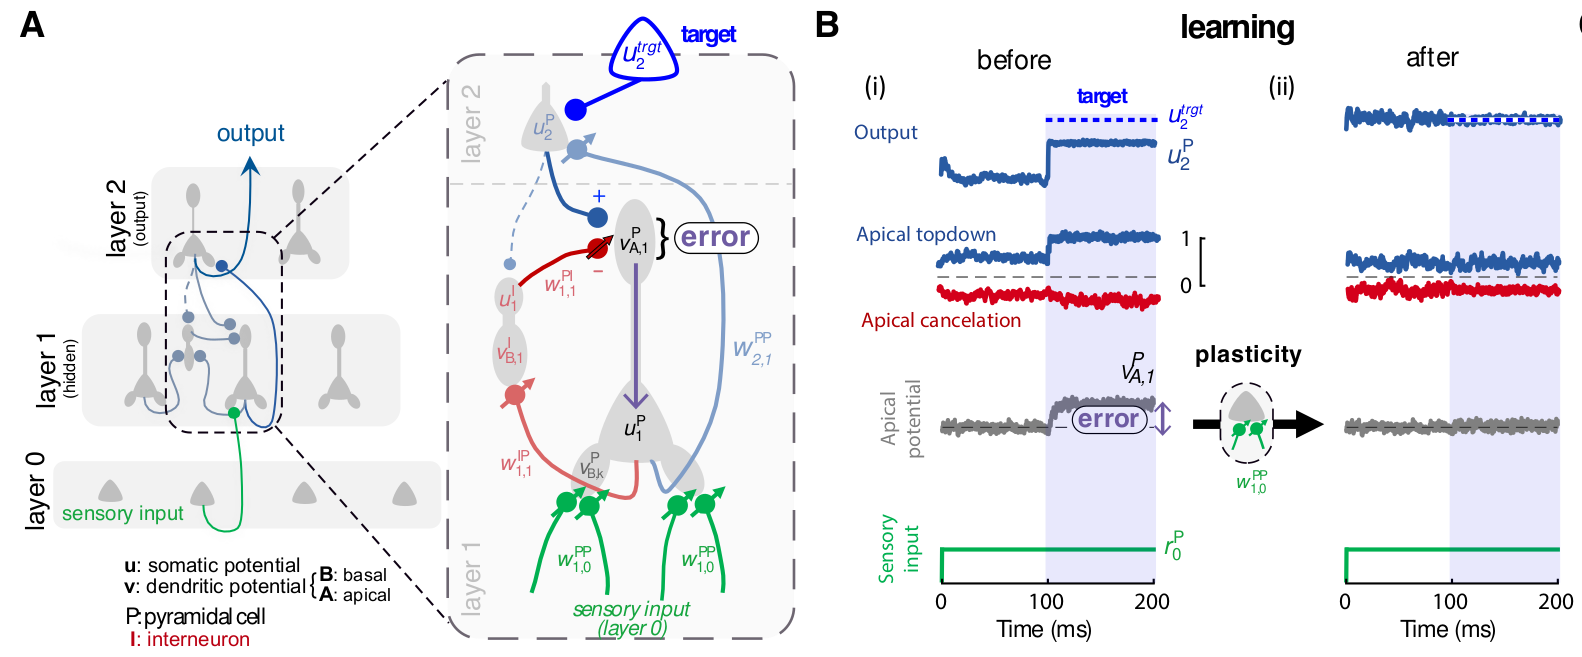
\includegraphics[width={1\linewidth}]{pyramidal.png}}
  \caption{Self-predicting initialization without plasticity}
\end{figure}
\section{Urbanczik-Senn Plasticity}


from \cite{Haider2021}:

\textit{In this architecture, plasticity serves two purposes. For pyramidal-to-pyramidal feedforward synapses,
  it implements error-correcting learning as a time-continuous approximation of BP. For pyramidal-to-
  interneuron synapses, it drives interneurons to mimic their pyramidal partners in the layers above (see
  also SI). Thus, in a well-trained network, apical compartments of pyramidal cells are at rest, reflecting
  zero error, as top-down and lateral inputs cancel out. When an output error propagates through the
  network, these two inputs can no longer cancel out and their difference represents the local error ei .
  This architecture does not rely on the transpose of the forward weight matrix, improving viability for
  implementation in distributed asynchronous systems. Here, we keep feedback weights fixed, realizing
  a variant of feedback alignment. In principle, these weights could also be learned in order to further
  improve the local representation of errors Section 7.}




One-sided exponential decay kernel

\begin{align}
  \kappa(t) & = H(t)e^{-t/\tau_{\kappa}} \\
  H(t)      & =
  \begin{cases}
    1 & \text{if $t > 0$}    \\
    0 & \text{if $t \leq 0$} \\
  \end{cases}
\end{align}

Antiderivatives:

\begin{align}
  \int_{-\infty}^x H(t)dt = tH(t) = max(0,t)
\end{align}

Convolution:

\begin{align*}
  (f \ast g)(t) & = \int_{- \infty }^{\infty} f(\tau) g(t-\tau) d \tau
\end{align*}
For functions f, g supported on only $[0, \infty]$ (as one-sided decay kernels and spiketrains are), integration limits can be truncated:
\begin{align*}
  (f \ast g)(t) & = \int_{0}^{t} f(\tau) g(t-\tau) d \tau \\
\end{align*}


Plasticity:

\begin{align}
  \frac{dW_{ij}}{dt}(t) & = F(W_{ij}(t), s_i^\ast (t), s_j^\ast (t), V_i^\ast (t)) \\
  F[s_j^\ast, V_i^\ast] & = \eta \kappa \ast (V_i^\ast s_j^\ast)                   \\
  \text{with } V_i^\ast & = (s_i - \phi(V_i )) h(V_i),                             \\
  s_j^\ast              & = \kappa_s \ast s_j.
\end{align}

For an event-based plasticity we need:

\begin{align}
  \Delta W_{ij}(t,T) & = \int_t^T dt' F[s_j^\ast , V_i^\ast ](t')                                                 \\
                     & = \int_t^T dt' \eta \kappa \ast (V_i^\ast s_j^\ast)                                        \\
                     & = \eta \int_t^T dt' \  \int_0^{t'} dt'' \ \kappa(t'-t'') V_i^\ast (t'') s_j^\ast (t'')     \\
                     & = \eta \int_0^t dt' \  \int_{t''}^{t'} dt'' \ \kappa(t'-t'') V_i^\ast (t'') s_j^\ast (t'') \\
\end{align}


Starting with the complete Integral from $t=0$.

\begin{align*}
  \Delta W_{ij}(0,t) & =\eta \int_0^t dt' \  \int_0^{t'} dt'' \ \kappa(t'-t'') V_i^\ast (t'') s_j^\ast (t'')                          \\
                     & = \eta \int_0^t dt'' \  \int_{t''}^{t} dt' \ \kappa(t'-t'') V_i^\ast (t'') s_j^\ast (t'')                      \\
                     & = \eta \int_0^t dt'' \  \left[ \tilde{\kappa}(t-t'') - \tilde{\kappa}(0) \right] V_i^\ast (t'') s_j^\ast (t'') \\
\end{align*}

With $\tilde{\kappa}$ being the antiderivative of $\kappa$:

\begin{align*}
  \kappa(t)         & = \frac{\delta}{\delta t} \tilde{\kappa}(t) \\
  \tilde{\kappa}(t) & = - e^{-\frac{t}{t_{\kappa}}}               \\
\end{align*}

The above can be split up into two separate integrals:
\begin{align*}
  \Delta W_{ij}(0,t) & =\eta \left[ -I_2 (0, t) + I_1(0,t) \right]                                      \\
  I_1(t_1, t_2)      & = - \int_{t_1}^{t_2} dt' \ \tilde{\kappa} (0) V_i^\ast (t') s_j^\ast (t')        \\
  I_2(t_1, t_2)      & = - \int_{t_1}^{t_2} dt' \ \tilde{\kappa} (t_2 - t') V_i^\ast (t') s_j^\ast (t') \\
\end{align*}

Which implies the identities

\begin{align*}
  I_1(t_1, t_2 + \Delta t) & = I_1 (t_1, t_2) + I_1 (t_2, t_2 + \Delta t)                                       \\
  I_2(t_1, t_2 + \Delta t) & = e^{- \frac{t_2 - t_1}{\tau_{\kappa}}} I_2 (t_1, t_2) + I_2 (t_2, t_2 + \Delta t)
\end{align*}


\begin{align}
  I_2 (t_1, t_2 + \Delta t) & = -\int_{t_1}^{t_2 + \Delta t} dt' \ \tilde{\kappa} (t_2 + \Delta t - t') V_i^\ast (t') s_j^\ast (t')                                        \\
                            & = -\int_{t_1}^{t_2} dt' \ \left[ -e^{- \frac{t_2 + \Delta t - t'}{\tau_\kappa}} \right] V_i^\ast (t') s_j^\ast (t')
  -\int_{t_2}^{t_2 + \Delta t} dt' \ \left[ -e^{- \frac{t_2 + \Delta t - t'}{\tau_\kappa}} \right] V_i^\ast (t') s_j^\ast (t')                                             \\
                            & = -e^{- \frac{ \Delta t}{\tau_\kappa}} \int_{t_1}^{t_2} dt' \ \left[ -e^{- \frac{t_2 - t'}{\tau_\kappa}} \right] V_i^\ast (t') s_j^\ast (t')
  -\int_{t_2}^{t_2 + \Delta t} dt' \ \left[ -e^{- \frac{t_2 + \Delta t - t'}{\tau_\kappa}} \right] V_i^\ast (t') s_j^\ast (t')
\end{align}


Using this we can rewrite the weight change from $t$ to $T$ as:


\begin{align*}
  \Delta W_{ij}(t,T) & = \Delta W_{ij}(0,T) - \Delta W_{ij}(0,t)                                               \\
                     & = \eta [-I_2(0,T) + I_1(0,T) + I_2(0,t) - I_1(0,t)]                                     \\
                     & = \eta [I_1(t,T) - I_2(t,T) + I_2(0,t)\left( 1 - e^{- \frac{T-t}{\tau_\kappa}} \right)]
\end{align*}

The simplified \cite{sacramento2018dendritic} case would be:

\begin{align*}
  \frac{dW_{ij}}{dt} & = \eta (\phi(u_i) - \phi(\hat{v_i})) \phi(u_j)                                         \\
  \Delta W_{ij}(t,T) & = \int_t^T dt' \ \eta \  (\phi(u_i^{t'}) - \phi(\widehat{v_i^{t'}})) \  \phi(u_j^{t'}) \\
  \Delta W_{ij}(t,T) & = \eta \int_t^T dt' \  (\phi(u_i^{t'}) - \phi(\widehat{v_i^{t'}})) \ \phi(u_j^{t'})    \\
  V_i^*              & = \phi(u_i^{t'}) - \phi(\widehat{v_i^{t'}})                                            \\
  s_j^*              & = \kappa_s * s_j
\end{align*}


Where $s_i$ is the postsynaptic spiketrain and $V_i^*$ is the error between dendritic prediction and somatic rate and $h( u )$. The additional nonlinearity $h( u ) = \frac{d}{du} ln \  \phi(u)$ is ommited in our model \todo{should it though?}.



\begin{align}
  \tau_l & = \frac{C_m}{g_L} = 10 \\
  \tau_s & = 3
\end{align}

Writing membrane potential to history (happens at every update step of the postsynaptic neuron):

\begin{lstlisting}[language=C++, directivestyle={\color{black}}
                   emph={int,char,double,float,unsigned,exp},
                   emphstyle={\color{blue}}]

UrbanczikArchivingNode< urbanczik_parameters >::write_urbanczik_history(Time t, double V_W, int n_spikes, int comp)
{
	double V_W_star = ( ( E_L * g_L + V_W * g_D ) / ( g_D + g_L ) );
	double dPI = ( n_spikes - phi( V_W_star ) * Time::get_resolution().get_ms() )
      * h( V_W_star );
}\end{lstlisting}

I interpret this as:


\begin{align*}
  \int_{t_{ls}}^T dt' \ V_i^* & = \int_{t_{ls}}^T dt' \  (s_i - \phi(V_i )) h(V_i),               \\
  \int_{t_{ls}}^T dt' \ V_i^* & = \sum_{t=t_{ls}}^T \  (s_i(t) -  \phi(V_i^t ) \Delta t) h(V_i^t) \\
\end{align*}

\begin{lstlisting}[language=C++, directivestyle={\color{black}}
                   emph={int,char,double,float,unsigned,exp},
                   emphstyle={\color{blue}}]
for (t = t_ls; t< T; t = t + delta_t)
{
   	minus_delta_t = t_ls - t;
    minus_t_down = t - T;
    PI = ( kappa_l * exp( minus_delta_t / tau_L ) - kappa_s * exp( minus_delta_t / tau_s ) ) * V_star(t);
    PI_integral_ += PI;
    dPI_exp_integral += exp( minus_t_down / tau_Delta_ ) * PI;
}  
// I_2 (t,T) = I_2(0,t) * exp(-(T-t)/tau) + I_2(t,T)
PI_exp_integral_ = (exp((t_ls-T)/tau_Delta_) * PI_exp_integral_ + dPI_exp_integral);
W_ji = PI_integral_ - PI_exp_integral_;
W_ji = init_weight_ + W_ji * 15.0 * C_m * tau_s * eta_ / ( g_L * ( tau_L - tau_s ) );    
  
kappa_l = kappa_l * exp((t_ls - T)/tau_L) + 1.0;
kappa_s = kappa_s * exp((t_ls - T)/tau_s) + 1.0;
  \end{lstlisting}


\begin{align*}
  \int_{t_{ls}}^T dt' s_j^* & =  \tilde{\kappa_L}(t') * s_j -  \tilde{\kappa_s}(t') * s_j
\end{align*}

$I_1$ in the code is computed as a sum:

\begin{align}
  I_1 (t,T) = \sum_{t'=t}^T \ (s_L^*(t') - s_s^*(t')) * V^*(t')
\end{align}


\section{steady-state potentials in Sacramento (2018)}

\begin{align*}
  u_k^p           & = \frac{g_B}{g_{lk} + g_B + g_A} v^P_{B,k} + \frac{g_A}{g_{lk} + g_B + g_A} v^P_{A,k} \\
  \hat{v}^P_{B,k} & = \frac{g_B}{g_{lk} + g_B + g_A} v^P_{B,k}                                            \\
  \hat{v}^I_{k}   & = \frac{g_B}{g_{lk} + g_B} v^I_{k}                                                    \\
  \lambda         & = \frac{g_{som}}{g_{lk} + g_B + g_{som}}
\end{align*}


\section{Haider 2021 updates}

Besides the using a prediction of future somatic activity for neuronal transfer and plasticity, \cite{Haider2021} also
slightly alter the plasticity rule, which turns out to be crucial for the latent equilibrium mechanism. While the 
simulations by \cite{sacramento2018dendritic} use the equations above, the new implementation \href{https://github.com/neurips}{fill with neurips link}
implicitly change them within its code. The fundamental building block of a network here is a layer, which is 
represented in code as an instance of the class \texttt{Layer}. Each instances holds information about its corresponding 
pyramidal- and interneurons. It also holds information about the synaptic connections between the two populations, as
well as all incoming feedforward and feedback pyramidal synapses. A layer has two class methods that are fundamental 
to its computation; \texttt{update()} computes membrane potential derivatives and synaptic weight changes given pyramidal
neuron activations from the previous and subsequent layers. \texttt{apply()} updates weights and membrane potentials 
from the previously calculated changes. Layers are processed in order from input to output layer, where all of them
receive the \texttt{update()} signal first, before \texttt{apply()} is called on all of them. This ordering ensures,
that changes in activation do not cascade through the layers and lead to excessive activations at the output. Yet, 
since next layer activations at time $t$ have not been computed, top down information is always delayed by one timestep.
\todo{evaluate importance of this}


Thus, the equations for membrane updates change slightly:

\begin{align*}
  \dot{W_{ij}}(t) & = \eta (\phi(u_i) - \phi(\alpha v^{basal}_i(t))) \phi(u_j)                                         \\
  \Delta W_{ij}(t,T) & = \int_t^T dt' \ \eta \  (\phi(u_i^{t'}) - \phi(\widehat{v_i^{t'}})) \  \phi(u_j^{t'}) \\
  \Delta W_{ij}(t,T) & = \eta \int_t^T dt' \  (\phi(u_i^{t'}) - \phi(\widehat{v_i^{t'}})) \ \phi(u_j^{t'})    \\
  V_i^*              & = \phi(u_i^{t'}) - \phi(\widehat{v_i^{t'}})                                            \\
  s_j^*              & = \kappa_s * s_j
\end{align*}



\section{Multi-compartment neuron models}



\section{Cortical microcircuits}

\section{Latent equilibrium}

\begin{align*}
  \phi(V^{som}) & \rightarrow \phi(\breve{V}^{som}) \\
  \breve{V}     & := V + \tau^m \dot{V}             \\
\end{align*}
\begin{align*}
  \frac{d}{dt} W_{ba} & = \eta (\phi(V_b^{som}) - \phi(\alpha V_b^{dend})) \phi(V_a^{som})                         \\
  \frac{d}{dt} W_{ba} & = \eta (\phi(\breve{V}_b^{som}) - \phi(\alpha \breve{V}_b^{dend})) \phi(\breve{V}_a^{som})
\end{align*}


\section{simulation details/updates}

All voltages need to be reset between simulations!



\chapter{Results}

The following results are exploratory in nature, and are 

\section{The self-predicting state}

As a first comparison between the three implmementations, the pre-training towards a self-predicting stat (cf.
\cite{sacramento2018dendritic} Figure S1) was performed with equal parametrizations, as shown in Figure
\ref{fig-self-pred}. For this experiment, no target signal is provided at the output layer, and the network was
stimulated with random inputs.



\begin{figure}[t]
    \centering
    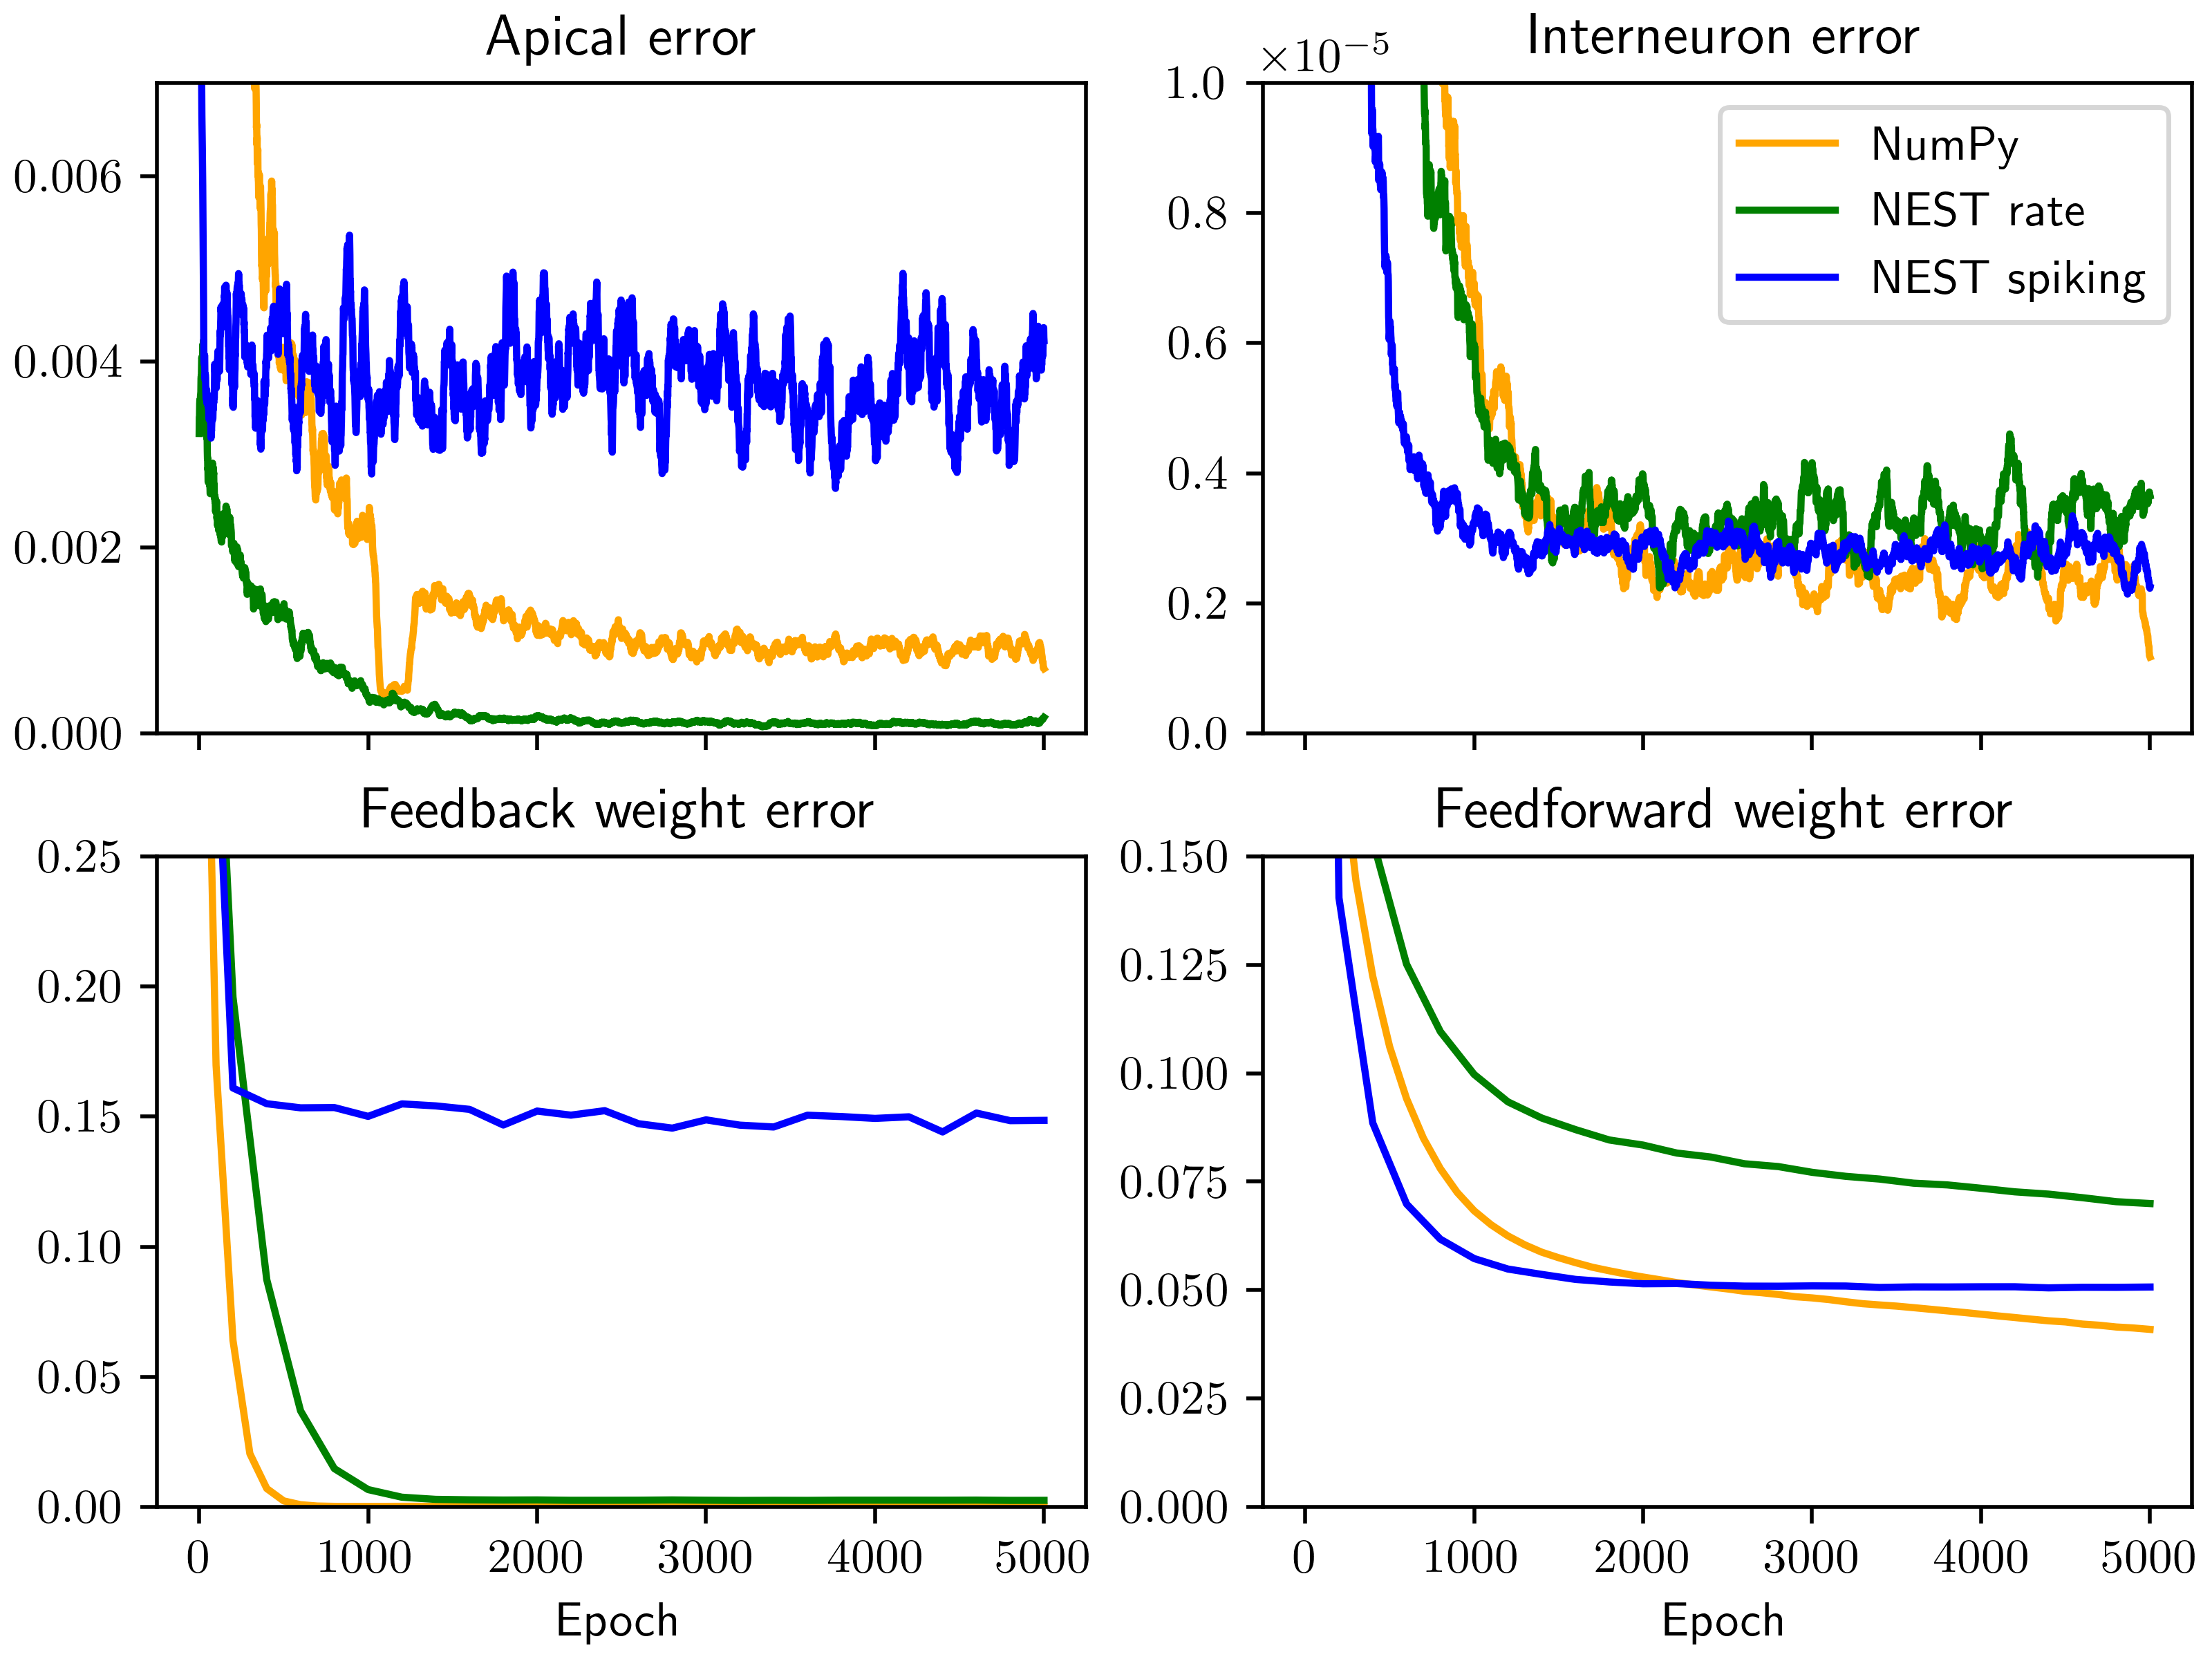
\includegraphics[width=0.9\textwidth]{fig_self_prediction}
    \caption{Different network types learn to predict self-generated activity in superficial layers. All networks were
        initialized with the same random weights for dimensions $[6, 10, 3]$, and stimulated with $5000$ samples of random input for $100ms$ each.
        As described in \cite{sacramento2018dendritic}, during only Pyramidal-Interneuron and Interneuron-Pyramidal
        weights are plastic ($\eta^{pi}=0.05, \eta^{ip}=0.02375, \eta^{up}=\eta^{down}=0$). All variants reach a
        self-predicting state within the first 1000 stimulus presentations and errors remain stable after that point.}
    \label{fig-self-pred}
\end{figure}

All implementations were able to reach comparable values for the four error metrics after roughly the same time. The
exact values that errors converge on differs slightly between implementations, but generally is on the same order of
magnitude and thus does not hinder learning performance greatly (cf. Section \ref{sec-le-tpres}). A notable outlier is
the apical error of pyramidal neuron in the spike-based implementation. This can however be traced back to individual
spikes causing substantial deviations in apical potentials, and can therefore be alleviated by increasing the
\textit{weight\_scale} parameter (results not shown) at the cost of increased training time. Alternatively, increasing
the membrane capacitance of the apical compartment also solves the issue as it smoothes out the effect of individual
spikes. Yet this solution also increases the relaxation period of the entire network, requiring a highly undesirable
increase in $t_{pres}$ for successful learning. Since weight errors converge to similar values as the rate-based
implementations, an increased absolute apical compartment voltage was deemed tolerable.



\section{Apical compartment capacitance}




\section{Presentation times with latent equilibrium}\label{sec-le-tpres}

In order to validate the performance of my implementations, I replicated a parameter study from \cite{Haider2021}[Fig.
    3]. The results for the NEST network using spiking neurons with default parameters \todo{elaborate on this} are
    shown in Figure \ref{fig-bars-le-snest}. A



\begin{figure}[t]
    \centering
    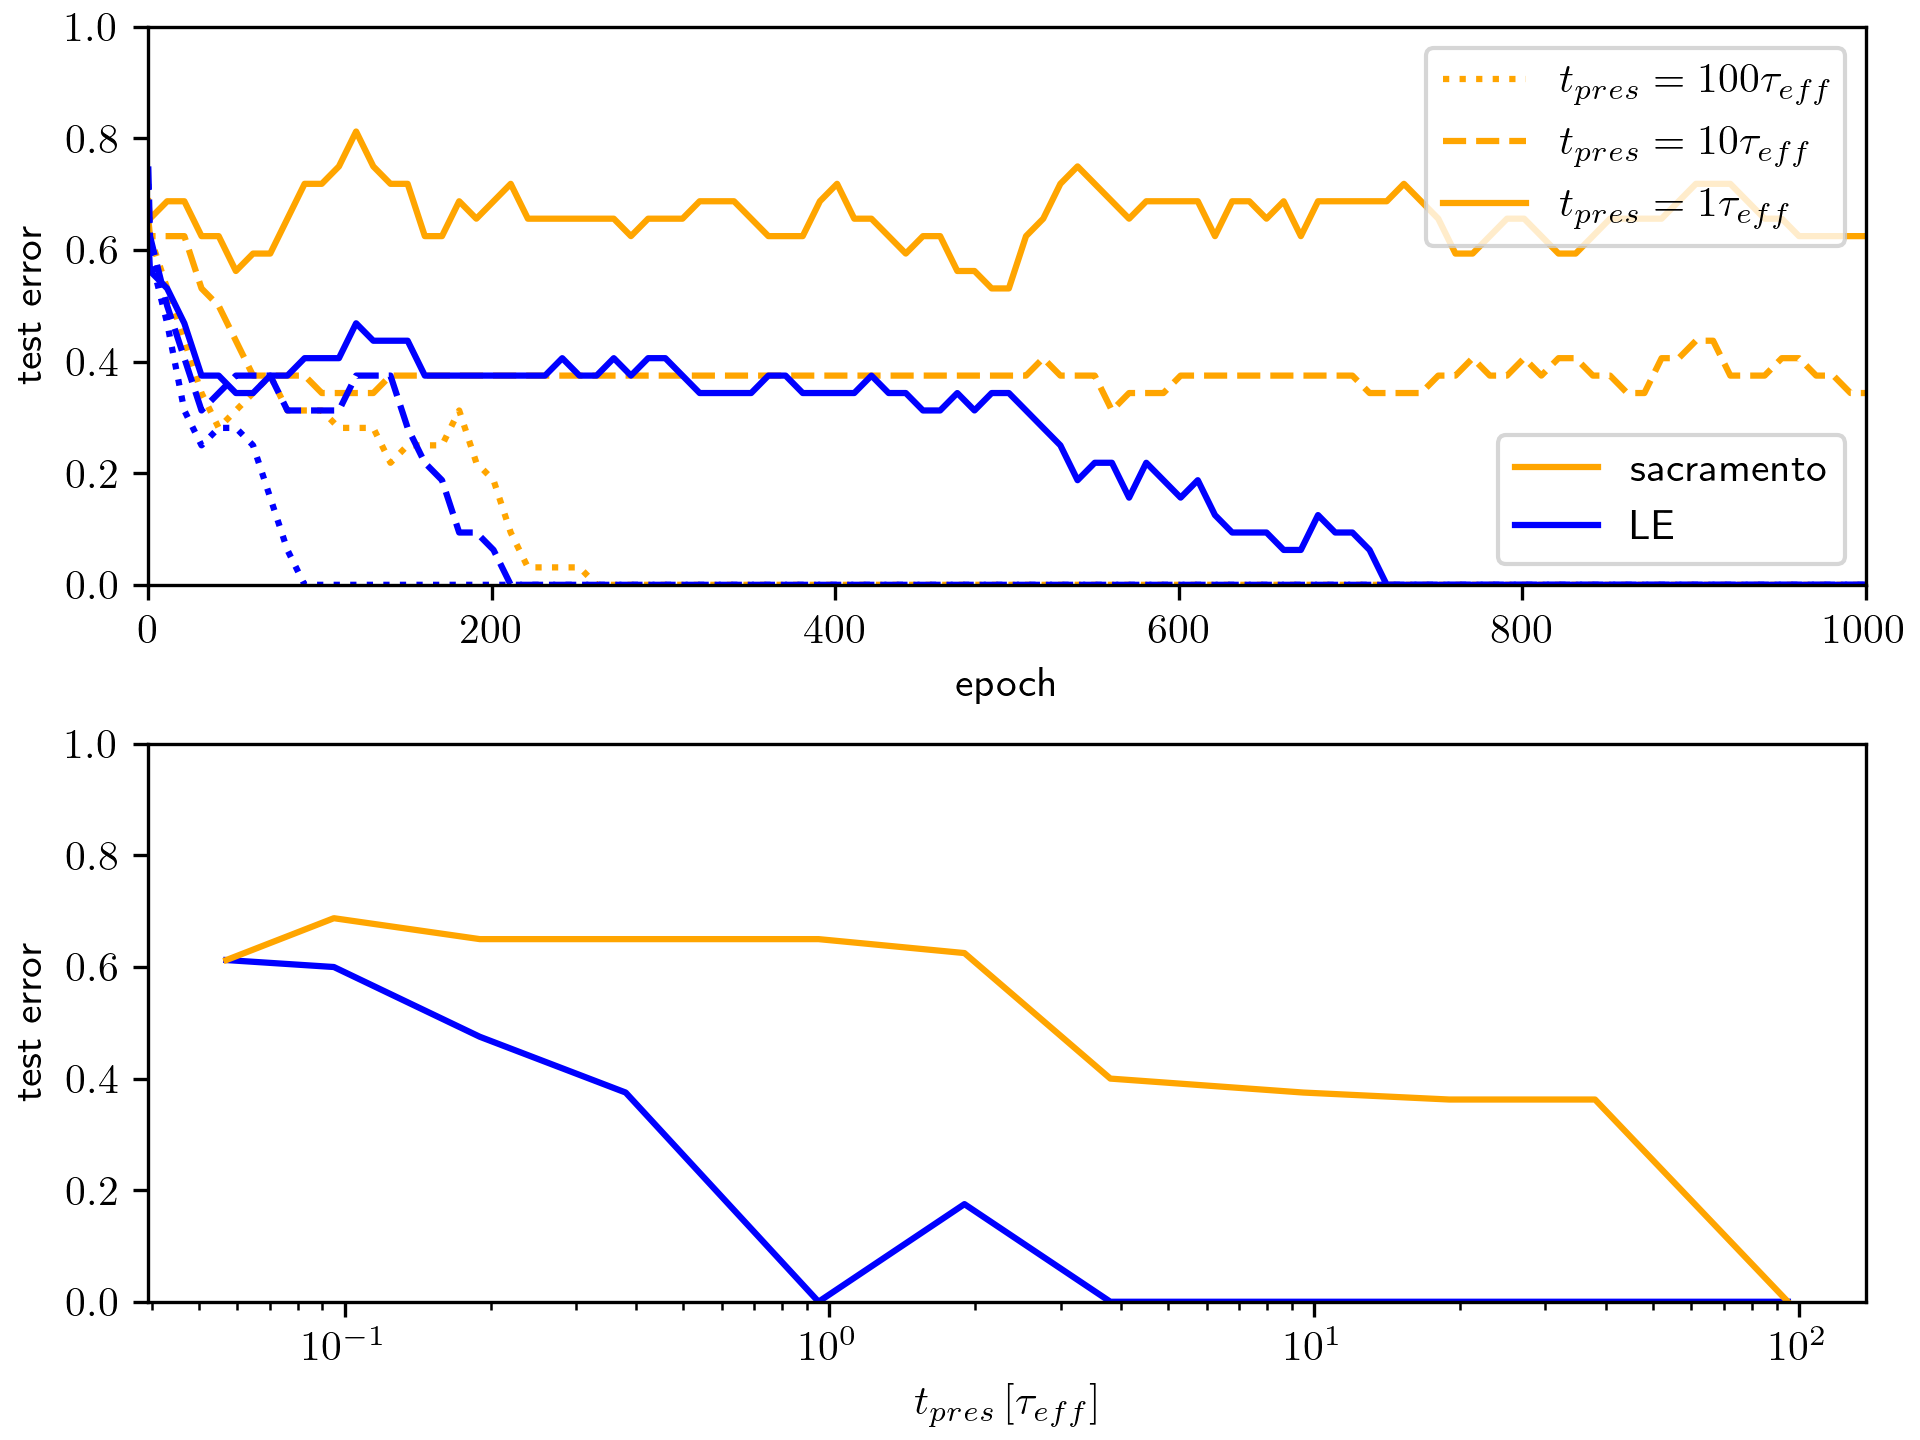
\includegraphics[width=0.9\textwidth]{fig_3_snest}
    \caption{Replication of Figure 3 from \cite{Haider2021} using networks of spiking neurons in the NEST simulator.
        \textbf{A:} Comparison between Original pyramidal microcircuit network by \cite{sacramento2018dendritic} and
        Latent equilibrium variant from \cite{Haider2021}. Shown is the training of a network with 9-30-3 neurons on the
        'Bars' Dataset from \todo{describe it} with three different stimulus presentation times. \textbf{B:} Test
        performance after 1000 Epochs as a function of stimulus presentation time.}
    \label{fig-bars-le-snest}
\end{figure}


\section{Separation of synaptic polarity}
\todo{investigate dales law \citep{Barranca2022}}

A key limitation of the present network model is the requirement that all synapses must be able to assume both positive
and negative polarities. When restricting any synaptic population in the network to just one polarity, the network is
unable to reach the self-predicting state \todo{expand?}. Thus, activity in any neuron must be able to have both
excitatory and inhibitory postsynaptic effects facilitated by appropriate synaptic weights. This requirement is at odds
with biology, which dictates a singular synaptic polarity for all outgoing connections of a neuron, determined by neuron
type and its corresponding neurotransmitter \citeme.


To investigate to what degree the plasticity rule can deal with this constraint, an experiment was conducted: A
 population of pyramidal neurons $A$  was connected to another population $C$ with plastic synapses that were
 constrained to positive weights. In order to facilitate the required depression, $A$ was also connected to a population
 of inhibitory interneurons $B$ through excitatory synapses with random and non-plastic weights. The interneurons in
 turn were connected to $C$ through plastic, inhibitory connections. All incoming synapses at $C$ targeted the same
 dendritic compartment. When inducing a dendritic error in that compartment, all plastic synapses in the network
 collaborated in order to minimize that error. When injecting a positive basal error for example, the inhibitory weights
 ($C \rightarrow B$) decayed, while excitatory synaptic weights ($A \rightarrow B$) increased. Flipping the sign of that
 error injection had the opposite effect on weights, and likewise cancelled the artificial error. This shows that a
 separation of synaptic polarity does not interfere with the principles of the Urbanczik-Senn plasticity when depression
 is facilitated by interneurons.

 \begin{figure}[t]
    \centering
    \begin{minipage}{0.2\textwidth}
        \textbf{a)}\par\medskip
        \centering
        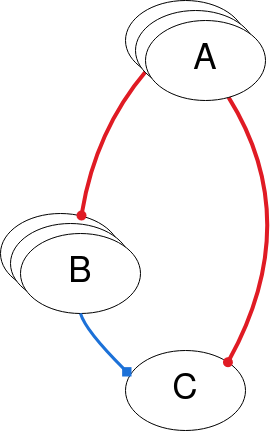
\includegraphics[width=0.9\textwidth]{fig_exc_inh_network}
    \end{minipage}\hfill
    \begin{minipage}{0.7\textwidth}
        \textbf{b)}\par\medskip
        \centering
        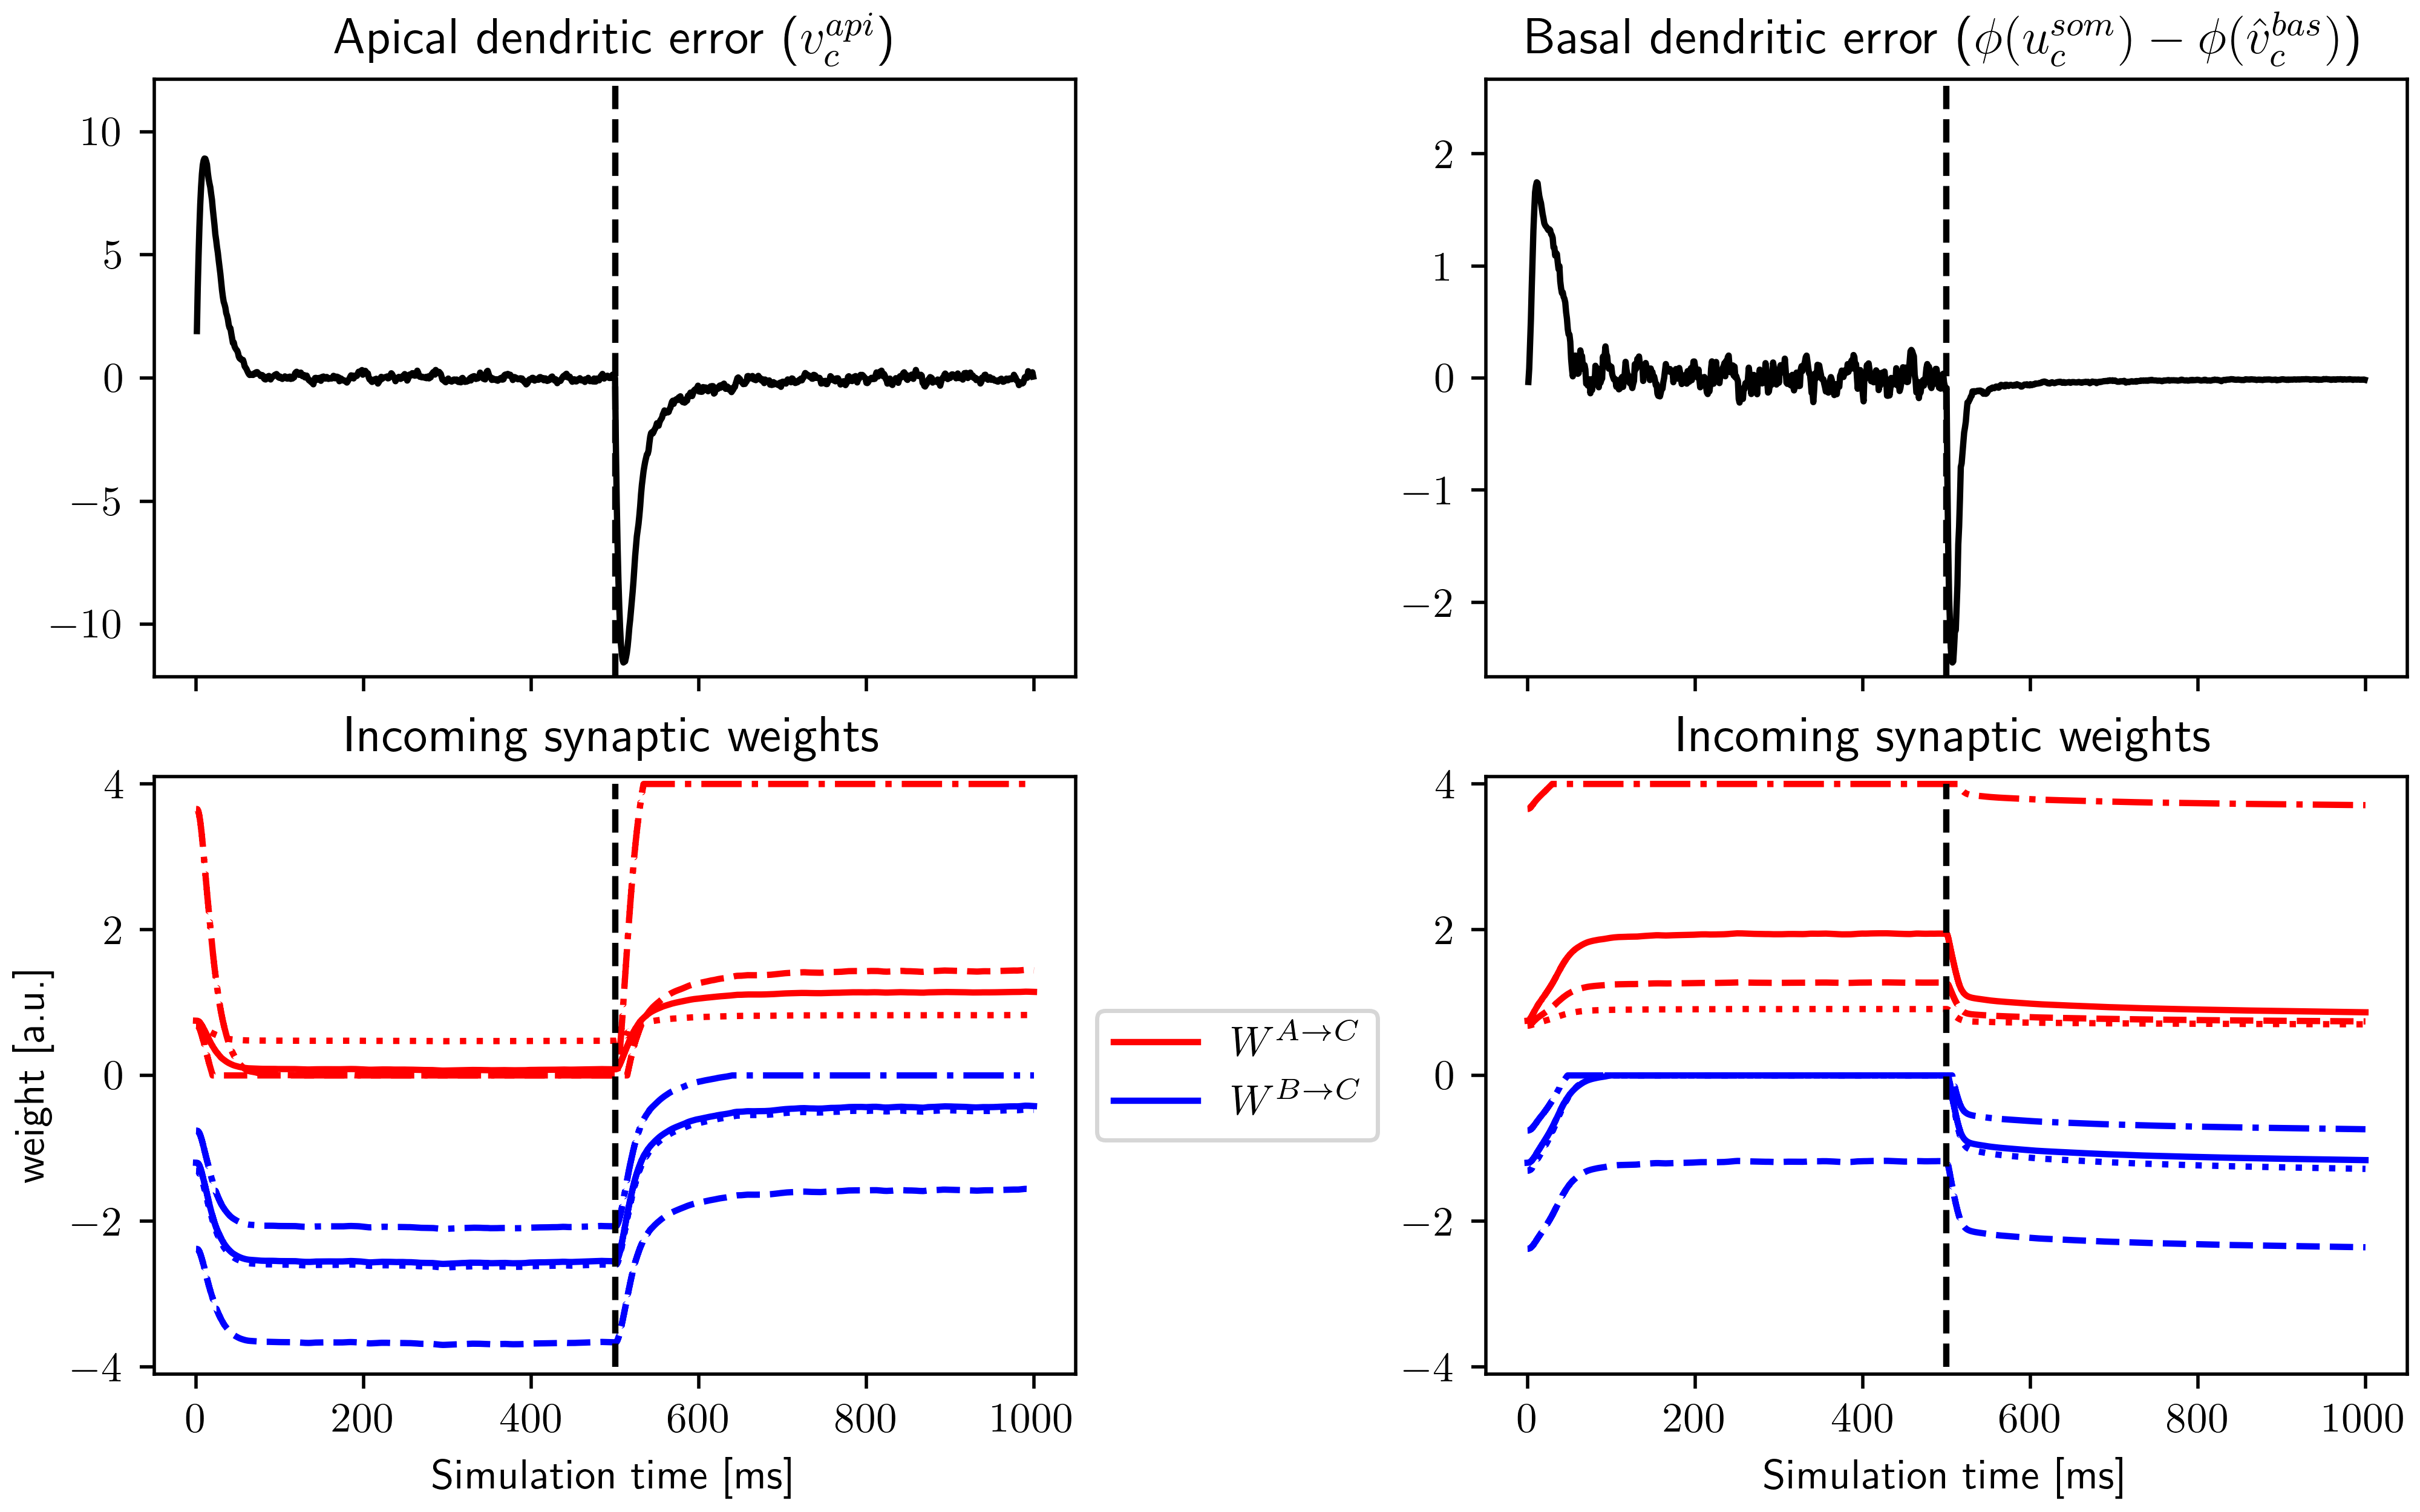
\includegraphics[width=0.9\textwidth]{fig_exc_inh_split}
    \end{minipage}
    \caption{Dendritic error minimization under biological constraints on synaptic polarity and network connectivity.
        \textbf{a)} Network architecture. An excitatory population $A$ connects to a dendrite of Neuron $C$ both
        directly and through inhibitory interneuron population $B$. Only synapses $A\rightarrow C$ and $B \rightarrow C$
        are plastic through dendritic error rules. Populations $A$ and $B$ are fully connected with random weights.
        \textbf{b)} \textit{Left:} All plastic synapses arrive at apical dendrites and evolve according to Equation
        \ref{eq-delta_w_pi}. \textit{Right:} Identical network setup, plasticity for synapses at basal dendrites
        (Equations \ref{eq-delta_w_up}, \ref{eq-delta_w_ip}). \textit{Top:} Dendritic error of a single target neuron.
        Errors of opposite signs are induced at $0$ and $500ms$ (vertical dashed line). \textit{Bottom:} Synaptic
        weights of incoming connections. All initial synaptic weights and input neuron activations were drawn from
        uniform distributions.}
    \label{fig-exc-inh-split}
\end{figure}

Yet, as criticised previously \citep{whittington2019theories}, the one-to-one connections between $A$ and $B$ are
untypical for biological neural networks \citeme. Hence, a second experiment was performed, in which $A$ and $B$ were
fully connected through static synapses with random positive weights. This decrease in specificity of the connections
did not hinder the error-correcting learning, as shown in Figure \ref{fig-exc-inh-split}.

These results are useful, as they enable a biologically plausible way for excitatory long-range pyramidal projections to
connect to pyramidal neurons in another layer (i.e. in a different part of the cortex). The steps required to facilitate
this type of network are rather simple; A pyramidal neuron projection could enter a distant cortical area and spread
spread its axonal tree \phrasing within a layer that contains both pyramidal neuron dendrites and interneurons. If these
interneurons themselves connect to the local pyramidal population, Errors with arbitrary signs and magnitudes in those
dendrites could be effectively minimized by the described connectivity. While error minimization is a funcamental
feature of this network, it does not necessarily imply that synaptic credit assignment is successful aswell. To prove
that this nonspecific connectivity does not hinder learning, it was introduced into the dendritic error network. The
connection between Interneurons and Pyramidal neuron apical dendrites was chosen for the first test, as the employed
plasticity rule had proven most resilient to parameter imperfections previously. A network of rate neurons was
initialized with self-predicting weights as in Section \ref{sec-le-tpres}. The Weights $w^{pi}$ were redrawn and
restricted to postive values, and a secondary inhibitory interneuron population was prepared and fully connected to both
populations as described in Figure \ref{fig-exc-inh-split}. 


\begin{figure}[t]
    \centering
    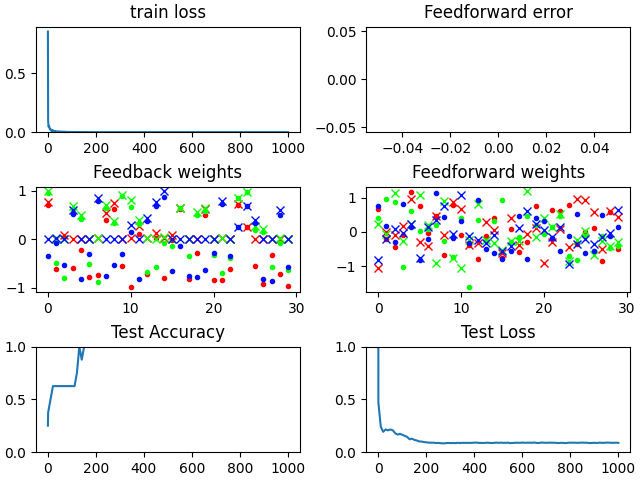
\includegraphics[width=0.8\textwidth]{fig_exc_inh_training}
    \caption{Training progress of a network of rate neurons in NEST, in which hidden layer connections between
    interneurons and pyramidal neurons are unipolar and nonspecific.}
    \label{fig-exc-inh-training}
\end{figure}


\section{In search of plausible spike frequencies}
 \todo{expand}


\section{Resilience to imperfect connectivity}

\begin{figure}[t]
    \centering
    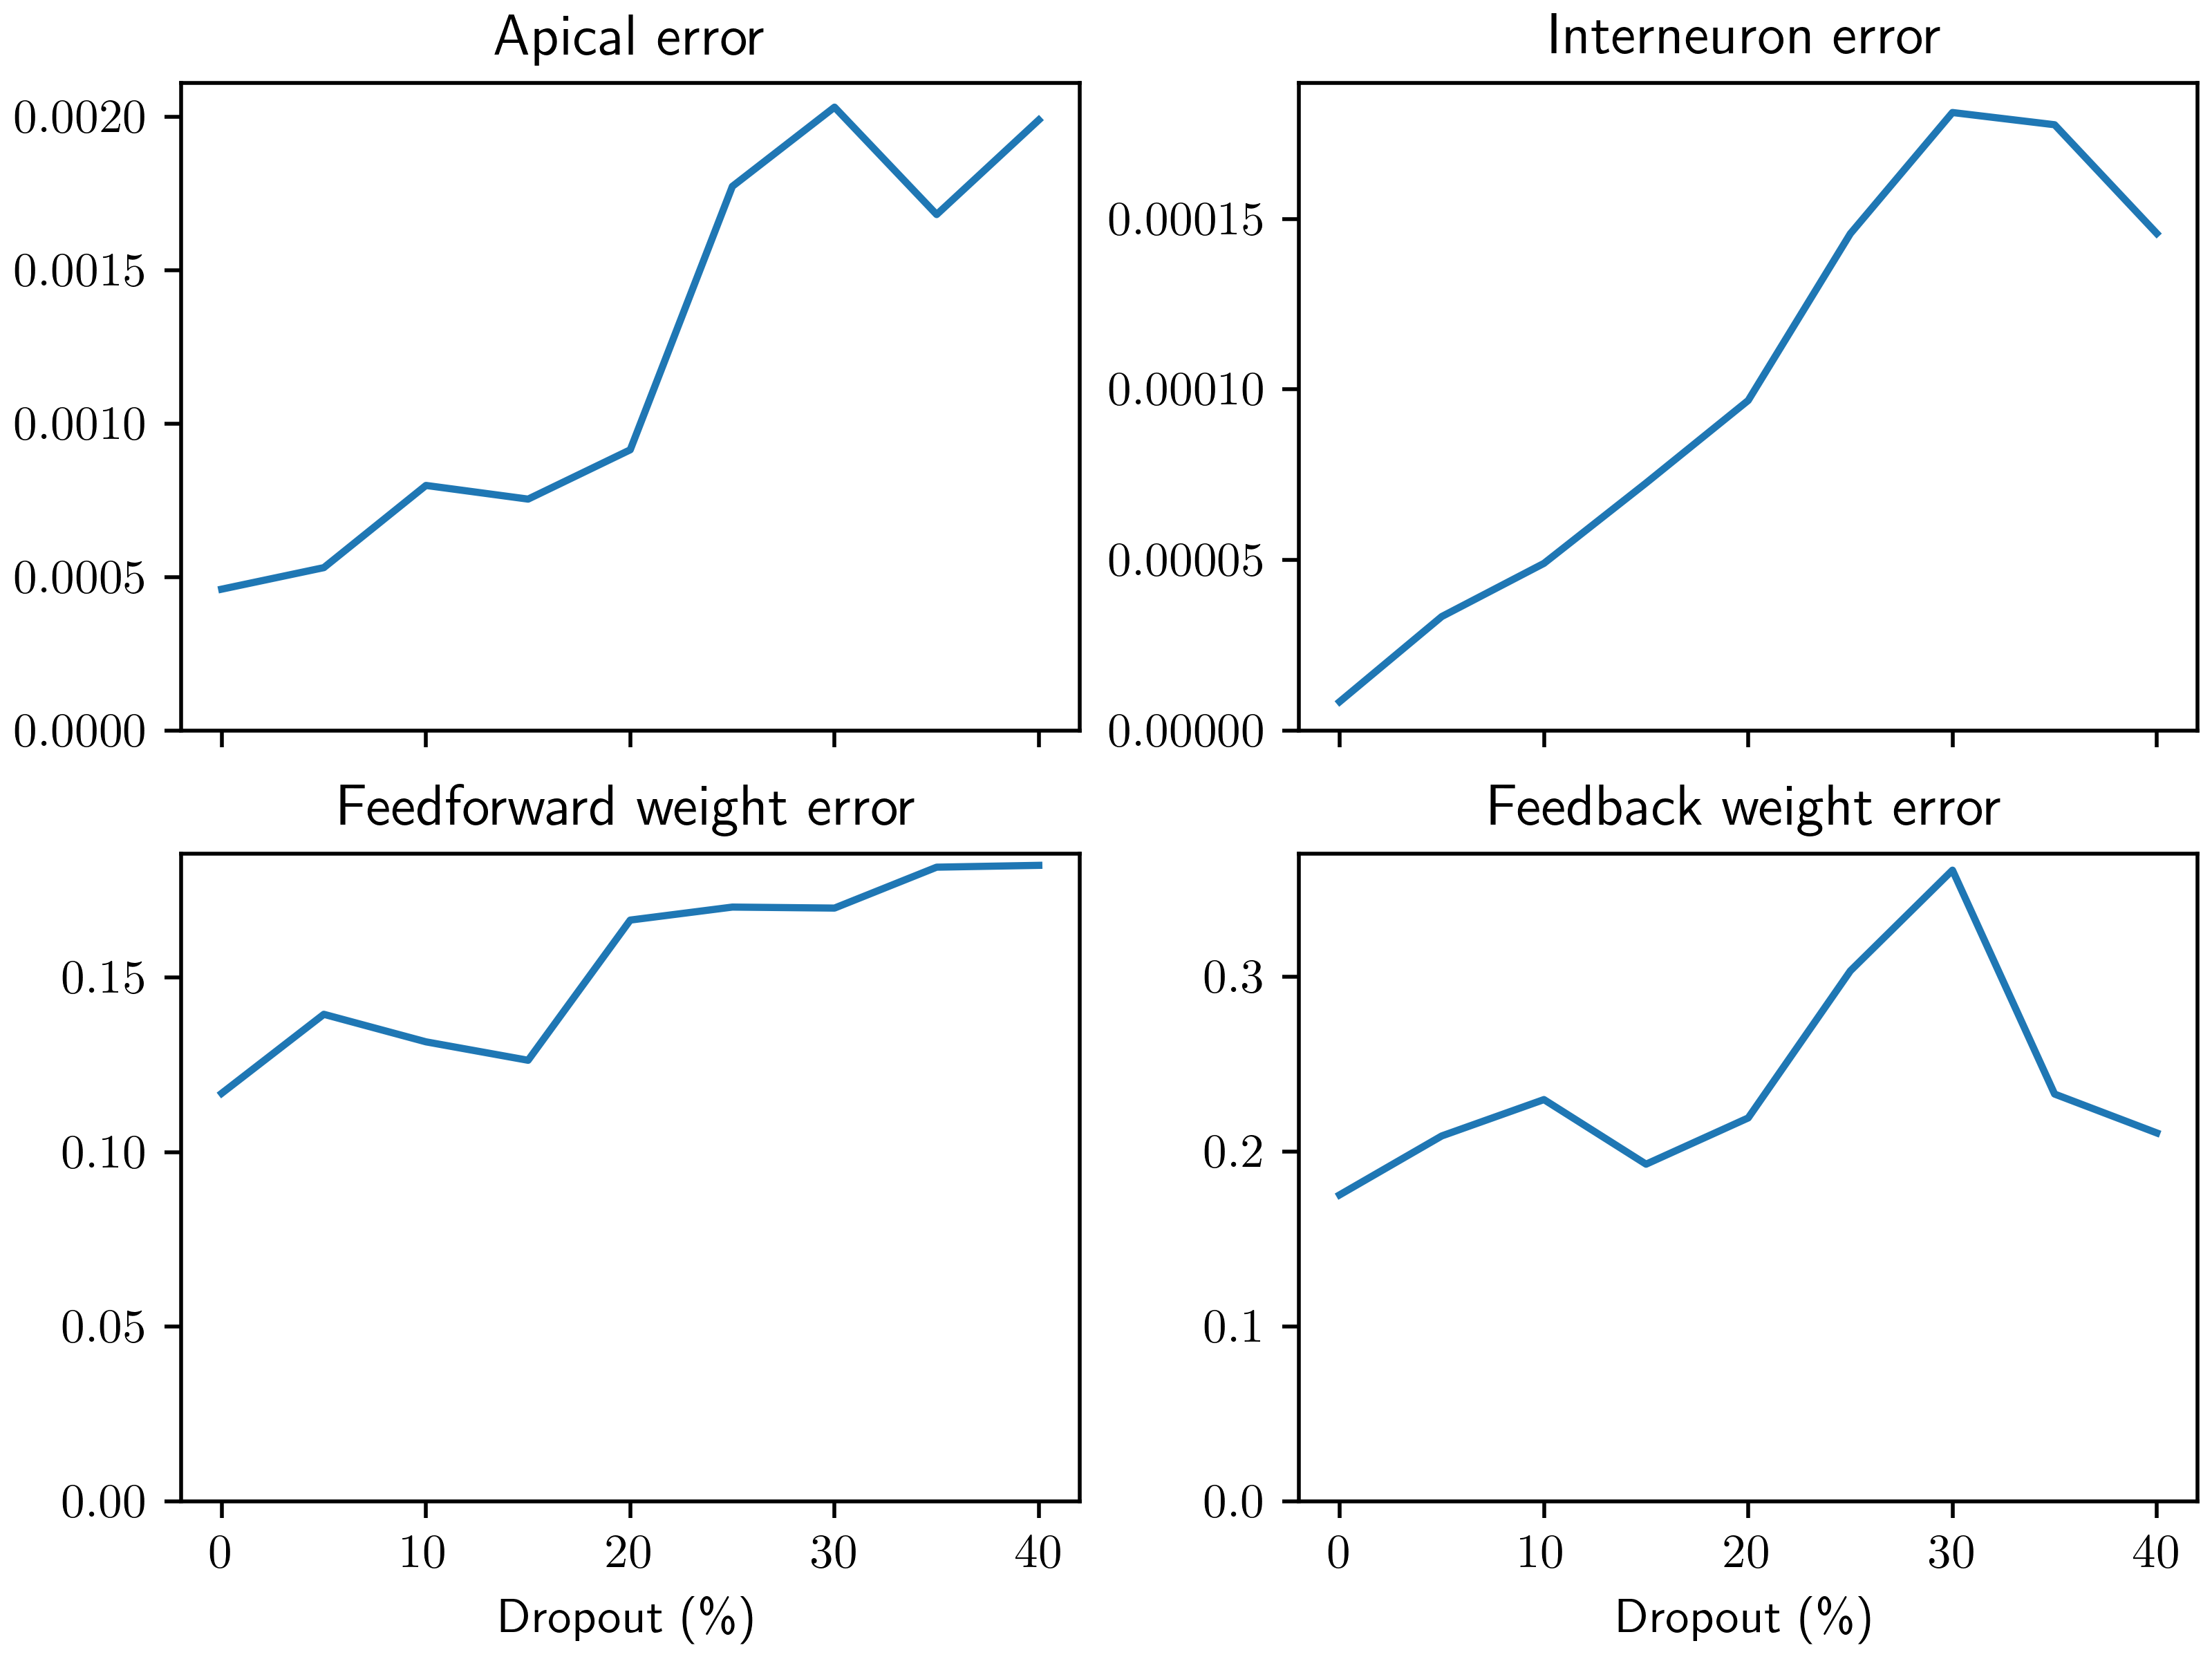
\includegraphics[width=0.9\textwidth]{fig_dropout}
    \caption{Error terms after training a network with dimensions [8, 8, 8] towards the self predicting states, with
    different percentages of synaptic connections randomly removed. To avoid completely separated layers, synapse
    deletion was performed per synaptic population, and the percentage is therefore only an approximation. Even with
    only 60\% of synaptic connections present, the network architecture still achieves competetive values for all four
    error metrics. For the weight errors, which is calculated with mean-squared-error over two matrices, missing
    synapses were set to $0$. This choice was made under the assumption that a missing connection in an ideal
    self-predicting network would be matched by a zero-weight - or likewise absent - synapse. Experiments were performed
    with the rate-based network in NEST, each network was trained fro 2000 epochs of 50ms each.}
    \label{fig-dropout}
\end{figure}


\section{direct feedback connections to interneurons}\label{sec-electric-syns}

\cite{Vaughn2022,Mancilla2007}



\section{Performance of the different implementations}

As stated in \cite{Haider2021}, simulating the present network with many neurons or more than one hidden layer quickly
becomes unfeasible when simulating the full leaky dynamics. To investigate how network size affects simulation time, all
three implementations created for this project were trained on the bars dataset for a single epoch with different
network sizes for a single epoch, in order to assess efficiency.


\begin{figure}[t]
    \centering
    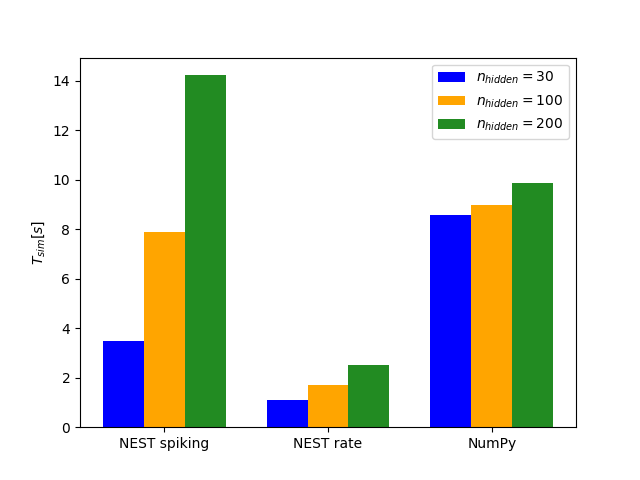
\includegraphics[width=0.8\textwidth]{fig_benchmark}
    \caption{Benchmark of the three different implementations using a network of $[9, n_{hidden}, 3]$ neurons per layer.
        $n_{hidden}=30$ was chosen as a baseline, as it is the default throughout all simulations on the Bars dataset.
        Networks were instantiated with the same synaptic weights and trained for a single epoch of 5 stimulus
        presentations of $100ms$ each. Simulations were performed on an \textit{AMD Ryzen Threadripper 2990WX} using 8
        cores for the NEST simulations at up to $3.0GHz$.}
    \label{fig-benchmark}
\end{figure}

The result of this comparison is shown in Figure \ref{fig-benchmark}. The NumPy network is slow at baseline, which is
likely explained by the fact that it is the only variant which is running on a single thread. This is due to a
limitation of NumPy, and could likely be improved greatly by using batched matrix multiplications, as are provided for
example by \texttt{PyTorch}\footnote{It is also possible, that the network code surrounding the NumPy computations is
less efficient than the one for the NEST network. As this implementation was needed primarily to prove that neuron
dynamics and synaptic updates were ported correctly to NEST, efficiency was a minor concern here and this was not
investigated further.}.  Notably, this variant exhibits very little slowdown in response to an increase in network size.
My assumption is, that the vectorization of synaptic updates on a single thread scales up better than the communication
between threads that is required by most events in the NEST simulations. The NEST implementation using rate neurons
performed best in terms of speed across the board. This result was slightly surprising, as the demand on the
communication interface between threads is very high, since all neurons transmit an event to each of their postsynaptic
targets at every time step.

Finally, the novel spiking variant of this model performed substantially worse than anticipated. Particularly in
comparison to the rate implementation, I initially expected substantial performance improvements. The Difference between
the two was even greater when simulating on an office-grade processor (Benchmark was also run on an \textit{Intel Core
i5-9300H} at $2.40GHz$, results not shown). Three hints about the comparatively poor performance can be deduced: For
one, both the rate and the spiking neuron model employ almost identical neuron models, with minor changes to
parametrization and output generation. Thus, updates to the neuron state are unlikely to be responsible for the worse
performance. Secondly, the number of Events transmitted between neurons is much lower for the SNN compared to

the \textit{relative} performance decrease when increasing the number neurons by the same amout is much greater for the
spiking network. Thus, the most likely cause of slowdown are the updates at the synapses. This is supported by the fact,
that the number of synapses increases much faster for this kind of network than the number of neurons. For the given
network of $n_{x} = 9$ input neurons, $n_y = 3$ output neurons and $n_{h}$ neurons in the hidden layer $l$, the number
of total synapses in the network is given by

\begin{align}
    n_{synapses} & = |w_{l}^{up}| + |w_{l}^{pi}| + |w_{l}^{ip}| + |w_{l}^{down}| + |w_{y}^{up}| \\
                 & = n_h n_x + n_h n_y + n_y n_h  + n_h n_y + n_y  n_h                          \\
                 & = n_h (n_x + n_y^4)
\end{align}

with $|w|$ of a weight matrix $w$ in this case denoting the total number of elements in that matrix \what{Is there a
    more conventional notation?}. Thus, the number of synapses in a network grows much faster than the number of total
    neurons when increasing the size of the hidden layer.

availis given by the stark increase in

\section{Response to unpredicted stimuli}

The activity of many cortical neurons increases when a brain is presented with unpredicted stimuly that regard these
neurons \todo{check out \cite{whittington2019theories} refs 50-54}. This property is prominently replicated by
predictive coding networks, since activation of error nodes is a function of local prediction errors. Prediction errors
in the present model on the other hand are encoded in both positive and negative potentials of apical dendrites. Hence, 
the 

\begin{figure}[t]
    \centering
    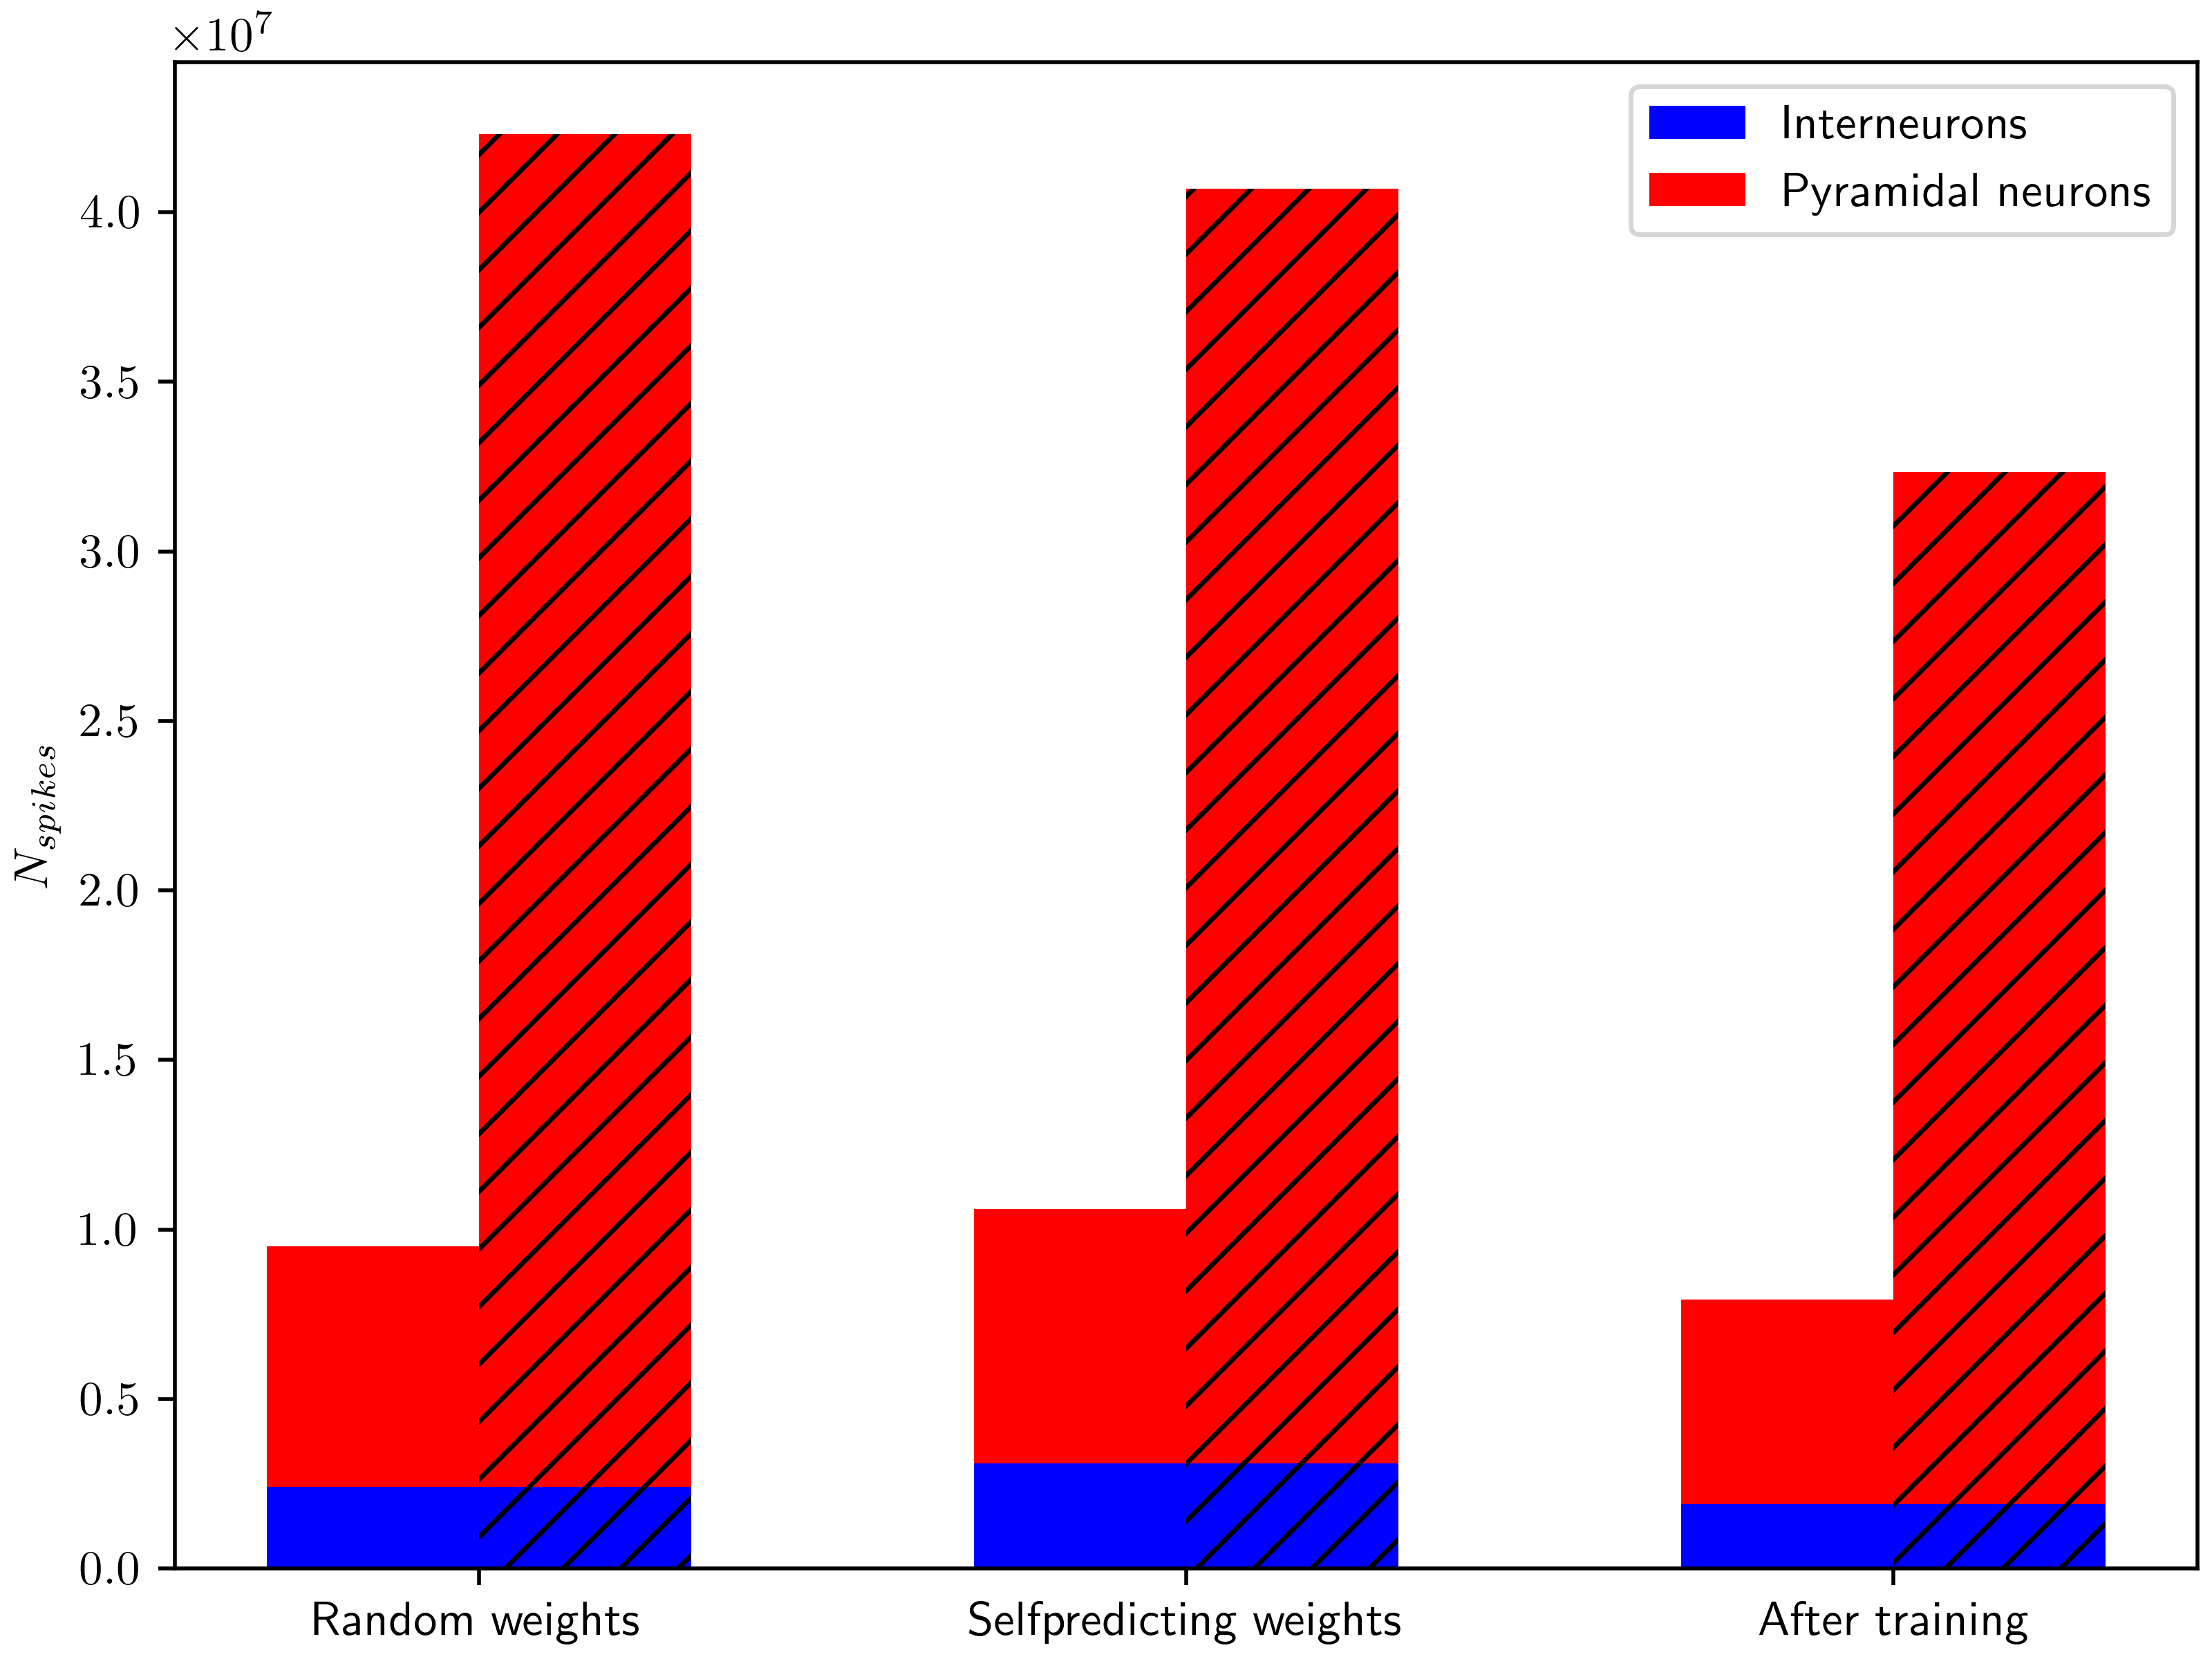
\includegraphics[width=0.9\textwidth]{fig_activity_unpredicted_stimulus}
    \caption{Comparison of network response to stimuli from the Bars dataset.}
    \label{fig-stimulus-response}
\end{figure}






\chapter{Discussion}


\section{Limitations of the implementation}

Network needs to be reset between stimuli
original does not do that, in NEST it's kindof a big deal.

exposure time and training set still quite large

non-resetting, non-refractory


\section{Whittington and Bogacz criteria}

In which we discuss, to what extent the network conforms to the criteria for biologically plausible learning rules
introduced by \cite{Whittington2017}:
\begin{enumerate}
    \item Local computation. A neuron performs computation only on the basis
          of the inputs it receives from other neurons weighted by the strengths
          of its synaptic connections.
    \item  Local plasticity. The amount of synaptic weight modification is dependent on only the activity of the two
          neurons the synapse connects (and possibly a neuromodulator).
    \item  Minimal external control. The neurons perform the computation autonomously with as little external control
          routing information in different ways at different times as possible.
    \item   Plausible architecture. The connectivity patterns in the model should
          be consistent with basic constraints of connectivity in neocortex.
\end{enumerate}



\section{Relation to energy minimization}

\section{Outlook}

reward-modulated urbanczik-senn plasticity?



\chapter{Appendix}



\section{Somato-dendritic coupling}\label{sec-somato-dendr}

\citep{urbanczik2014learning} discuss a possible extension to their neuron- and plasticity model, in which the
dendro-somatic coupling transmits voltages in both directions. They show that the plasticity rule requires only minor
adaptations for successful learning under this paradigm. Yet, as described by passive cable theory, the flow between
neuronal compartments is dictated by their respective membrane capacitances. These are calculated from their membrane
areas, which vastly differ in the case of pyramidal neurons. \todo{find a nice citation for this}


15,006 458


will not be considered here. The motivation is, that dendritic membrane area is



\section{Default parameters}

\section{Integration of the spike-based Urbanczik-Senn plasticity}



Starting with the complete Integral from $t=0$.

\begin{align}
  \dot{W_{ij}}(t)    & = \eta (\phi(u_i) - \phi(\alpha v^{basal}_i(t))) \phi(u_j)                                                     \\
  \Delta W_{ij}(t,T) & = \int_t^T dt' \ \eta \  (\phi(u_i^{t'}) - \phi(\widehat{v_i^{t'}})) \  \phi(u_j^{t'})                         \\
  \Delta W_{ij}(t,T) & = \eta \int_t^T dt' \  (\phi(u_i^{t'}) - \phi(\widehat{v_i^{t'}})) \ \phi(u_j^{t'})                            \\
  V_i^*              & = \phi(u_i^{t'}) - \phi(\widehat{v_i^{t'}})                                                                    \\
  s_j^*              & = \kappa_s * s_j                                                                                               \\
  \Delta W_{ij}(0,t) & =\eta \int_0^t dt' \  \int_0^{t'} dt'' \ \kappa(t'-t'') V_i^\ast (t'') s_j^\ast (t'')                          \\
                     & = \eta \int_0^t dt'' \  \int_{t''}^{t} dt' \ \kappa(t'-t'') V_i^\ast (t'') s_j^\ast (t'')                      \\
                     & = \eta \int_0^t dt'' \  \left[ \tilde{\kappa}(t-t'') - \tilde{\kappa}(0) \right] V_i^\ast (t'') s_j^\ast (t'') \\
\end{align}

With $\tilde{\kappa}$ being the antiderivative of $\kappa$:

\begin{align}
  \kappa(t)         & = \frac{\delta}{\delta t} \tilde{\kappa}(t) \\
  \tilde{\kappa}(t) & = - e^{-\frac{t}{t_{\kappa}}}               \\
\end{align}

The above can be split up into two separate integrals:

Which implies the identities

\begin{align}
  I_1(t_1, t_2 + \Delta t) & = I_1 (t_1, t_2) + I_1 (t_2, t_2 + \Delta t)                                       \\
  I_2(t_1, t_2 + \Delta t) & = e^{- \frac{t_2 - t_1}{\tau_{\kappa}}} I_2 (t_1, t_2) + I_2 (t_2, t_2 + \Delta t)
\end{align}


\begin{align}
  I_2 (t_1, t_2 + \Delta t) & = -\int_{t_1}^{t_2 + \Delta t} dt' \ \tilde{\kappa} (t_2 + \Delta t - t') V_i^\ast (t') s_j^\ast (t')                                        \\
                            & = -\int_{t_1}^{t_2} dt' \ \left[ -e^{- \frac{t_2 + \Delta t - t'}{\tau_\kappa}} \right] V_i^\ast (t') s_j^\ast (t')
  -\int_{t_2}^{t_2 + \Delta t} dt' \ \left[ -e^{- \frac{t_2 + \Delta t - t'}{\tau_\kappa}} \right] V_i^\ast (t') s_j^\ast (t')                                             \\
                            & = -e^{- \frac{ \Delta t}{\tau_\kappa}} \int_{t_1}^{t_2} dt' \ \left[ -e^{- \frac{t_2 - t'}{\tau_\kappa}} \right] V_i^\ast (t') s_j^\ast (t')
  -\int_{t_2}^{t_2 + \Delta t} dt' \ \left[ -e^{- \frac{t_2 + \Delta t - t'}{\tau_\kappa}} \right] V_i^\ast (t') s_j^\ast (t')
\end{align}


Using this we can rewrite the weight change from $t$ to $T$ as:


\begin{align}
  \Delta W_{ij}(t,T) & = \Delta W_{ij}(0,T) - \Delta W_{ij}(0,t)                                               \\
                     & = \eta [-I_2(0,T) + I_1(0,T) + I_2(0,t) - I_1(0,t)]                                     \\
                     & = \eta [I_1(t,T) - I_2(t,T) + I_2(0,t)\left( 1 - e^{- \frac{T-t}{\tau_\kappa}} \right)]
\end{align}

The simplified \citep{sacramento2018dendritic} case would be:

\begin{align}
  \frac{dW_{ij}}{dt} & = \eta (\phi(u_i) - \phi(\hat{v_i})) \phi(u_j)                                         \\
  \Delta W_{ij}(t,T) & = \int_t^T dt' \ \eta \  (\phi(u_i^{t'}) - \phi(\widehat{v_i^{t'}})) \  \phi(u_j^{t'}) \\
  \Delta W_{ij}(t,T) & = \eta \int_t^T dt' \  (\phi(u_i^{t'}) - \phi(\widehat{v_i^{t'}})) \ \phi(u_j^{t'})    \\
  V_i^*              & = \phi(u_i^{t'}) - \phi(\widehat{v_i^{t'}})                                            \\
  s_j^*              & = \kappa_s * s_j
\end{align}


Where $s_i$ is the postsynaptic spiketrain and $V_i^*$ is the error between dendritic prediction and somatic rate and
$h( u )$. The additional nonlinearity $h( u ) = \frac{d}{du} ln \  \phi(u)$ is ommited in our model \todo{should it
  though?}.




Antiderivatives:

\begin{align}
  \int_{-\infty}^x H(t)dt = tH(t) = max(0,t)
\end{align}


\begin{align}
  \tau_l & = \frac{C_m}{g_L} = 10 \\
  \tau_s & = 3
\end{align}

Writing membrane potential to history (happens at every update step of the postsynaptic neuron):



\section{Dendritic leakage conductance}\label{sec-gl-dend}

In order to match the dendritic potential of rate neurons  in the spiking neuron model, a suitable leakage conductance
for dendritic compartments was required. As described in Equation \ref{eq-spiking-basal-compartment}, a dendritic
compartment evolves according to:
\begin{align}
  C_m^{dend} \dot{v}_j^{dend} & = -g_l^{dend} \  v_j^{dend} + \sum_i W_{ji} \    \langle \textit{n}_i \rangle
\end{align}

Under the assumption that the activation of all presynaptic neurons $i$ remains static over time, we can replace the
spontaneous activation $s_i(t)$ with the expected number of spikes per simulation step $\langle \textit{n}_i \rangle =
  r_i \ \Delta t$ (cf. Equation \ref{eq-n-spikes}). Note that these values do not employ matrix notation, but refer to
individual neurons. Next, in order to find the convergence point of the ODE, we set the left side of the equation to $0$
and to solve it:

\begin{align}
  0                        & = -g_l^{dend} \  v_j^{dend} + \sum_i W_{ji} \    r_i \ \Delta t \\
  g_l^{dend} \  v_j^{dend} & = W_{ji} \    r_i \ \Delta t
\end{align}

The instantaneous dendritic potential of rate neurons is given by $v_j^{dend} = \sum_i W_{ji} \ r_i$. Since we are
searching for a parametrization which fulfils this equality in the steady state, the terms drop out from the above
equation. Thus, the correct parametrization for the dendritic leakage conductance remains:
\begin{align}
  g_l^{dend} & = \Delta t
\end{align}

It was shown experimentally that for high values of $\psi$, this parameterization leads to an exact match of dendritic
potentials between the neuron models. It will therefore be assumed as the default throughout all experiments where
spiking neurons are used. \newline

In order to keep the two NEST models as similar as possible, rate neurons evolve according to the same dynamics. Like in
the original implementation, dendrites of rate neurons ought to be fully defined by their inputs at time $t$. This
behaviour is achieved by setting the leakage conductance to $1$ for all dendritic compartments. During network
initialization, dendritic leakage conductances are set to either one of these values depending on the type of neuron
model employed.


\section{Plasticity in feedback connections}\label{sec-feedback-plast}

\todo{move to results}

Within the present model, Pyramidal-to-pyramidal feedback weights evolve according to:

\begin{align}
  \dot{w}_{l}^{down} & = \eta_l^{down} \ ( \phi(u_l^{P}) - \phi(w_l^{down} r_{l+1}^P) )\ \phi(u_{l+1}^{P})^T
\end{align}

The error term in this case differs slightly from the others, but could arguably still be implemented by biological
neurons. An intuitive way to interpret the error term is as the difference between somatic activity and the activity of
a distant apical compartment that is innervated only by superficial pyramidal neurons. Within the NEST implementation,
this distal compartment leaks into the proximal apical compartment ($v^{api}$) with a conductance of $g^{api,dist}=1$.
The separation of pyramidal neuron apical dendrites into a proximal and a distal tree is well documented \citeme. A
difference between plasticity mechanisms for synapses arriving at these two integration zones is plausible, although I
was unable to find prior research supporting this type of plasticity \citeme.  A more sophisticated model of the apical
tree which resembles pyramidal neurons more closely could be a desirable extension to the model.

While the plasticity was successfully implemented in all variants of the model, it did not prove useful for training the
networks during initial tests. A strong indicator to the reason behind this is the fact, that the dendritic error for
this rule is nonzero, even in the self-predicting state (cf. Fig. \ref{fig-error-comp-le}). Making these connections
non-plastic led to the best learning performance, and is therefore assumed as the default for all training simulations.
This matches the previous implementations of this network too, which typically set learning rates of these connections
to $0$ with the exception of a few experiments employing steady-state approximations. Note that feedback information is
transmitted through fixed weights in this case. Feedforward weights in turn learn to match these, meaning that the
network effectively implements a type of Feedback alignment \citep{Lillicrap2014}.

\newpage
\section{Supplementary Figures}


\renewcommand{\thefigure}{S\arabic{figure}}
\begin{figure}[h!]
  \centering
  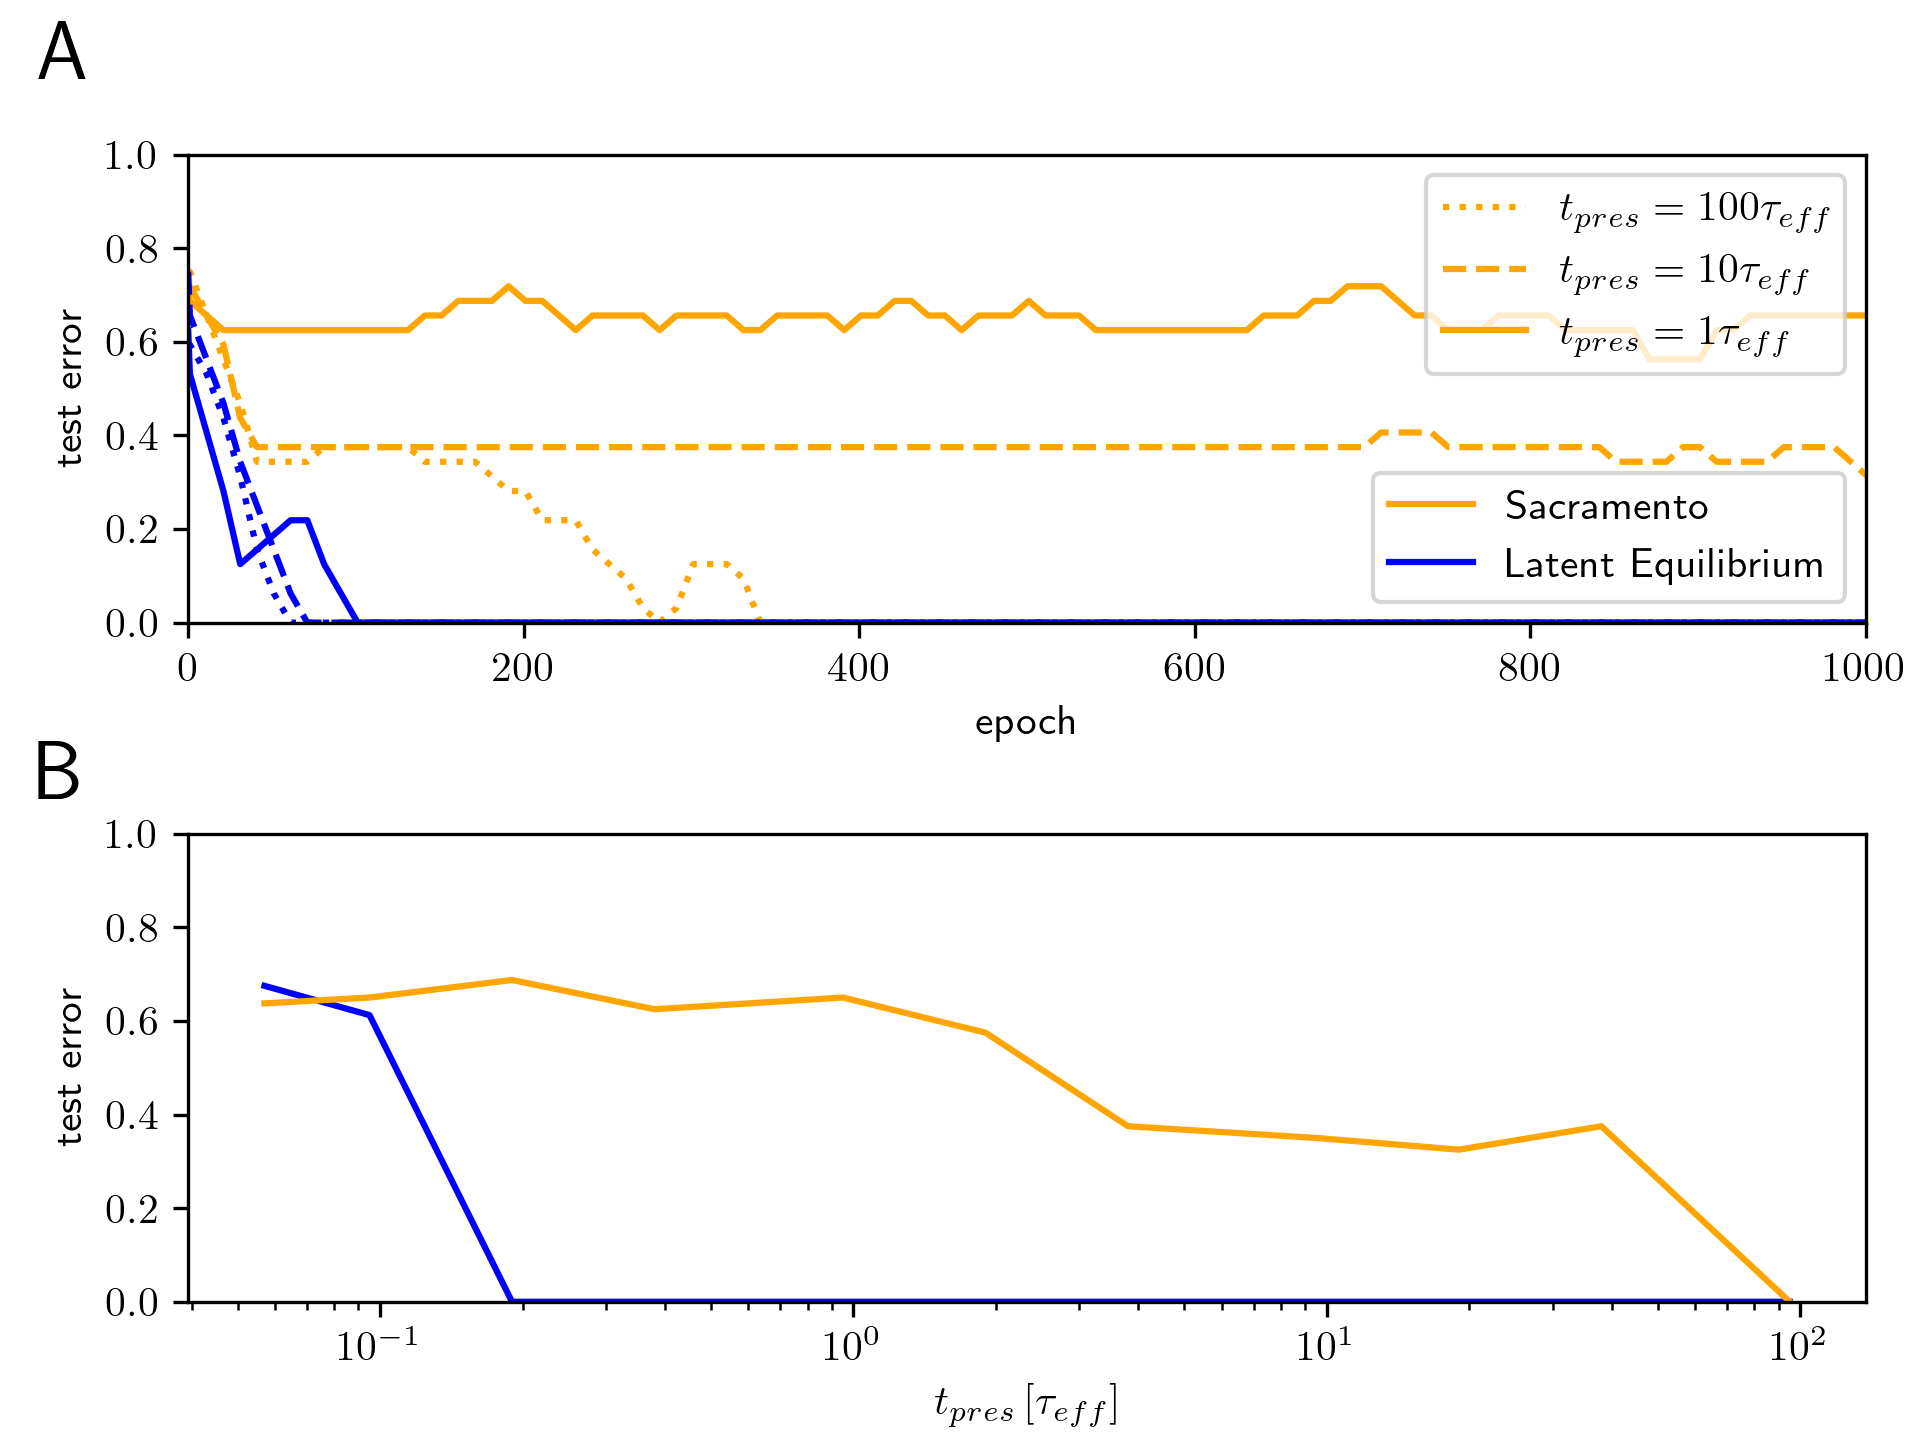
\includegraphics[width=0.9\textwidth]{fig_3_numpy}
  \caption[Replication of Fig. \ref{fig-bars-le-snest} using the NumPy network]{Replication of Fig.
    \ref{fig-bars-le-snest} using the NumPy network. This varaint is a slightly modified version of the python code from
    \citep{Haider2021}. Resulting performance matches the original results closely, showing that this version can serve
    as a baseline for comparing performance of the NEST implementation to the original results. Note, how in this
    implementation, presentation time has hardly any effect on the LE network because all updates are instantaneous. At
    the lower end presentation time is only limited by simulation timestep $\Delta t$.}
  \label{fig-bars-le-numpy}
\end{figure}


\begin{figure}[h!]
  \centering
  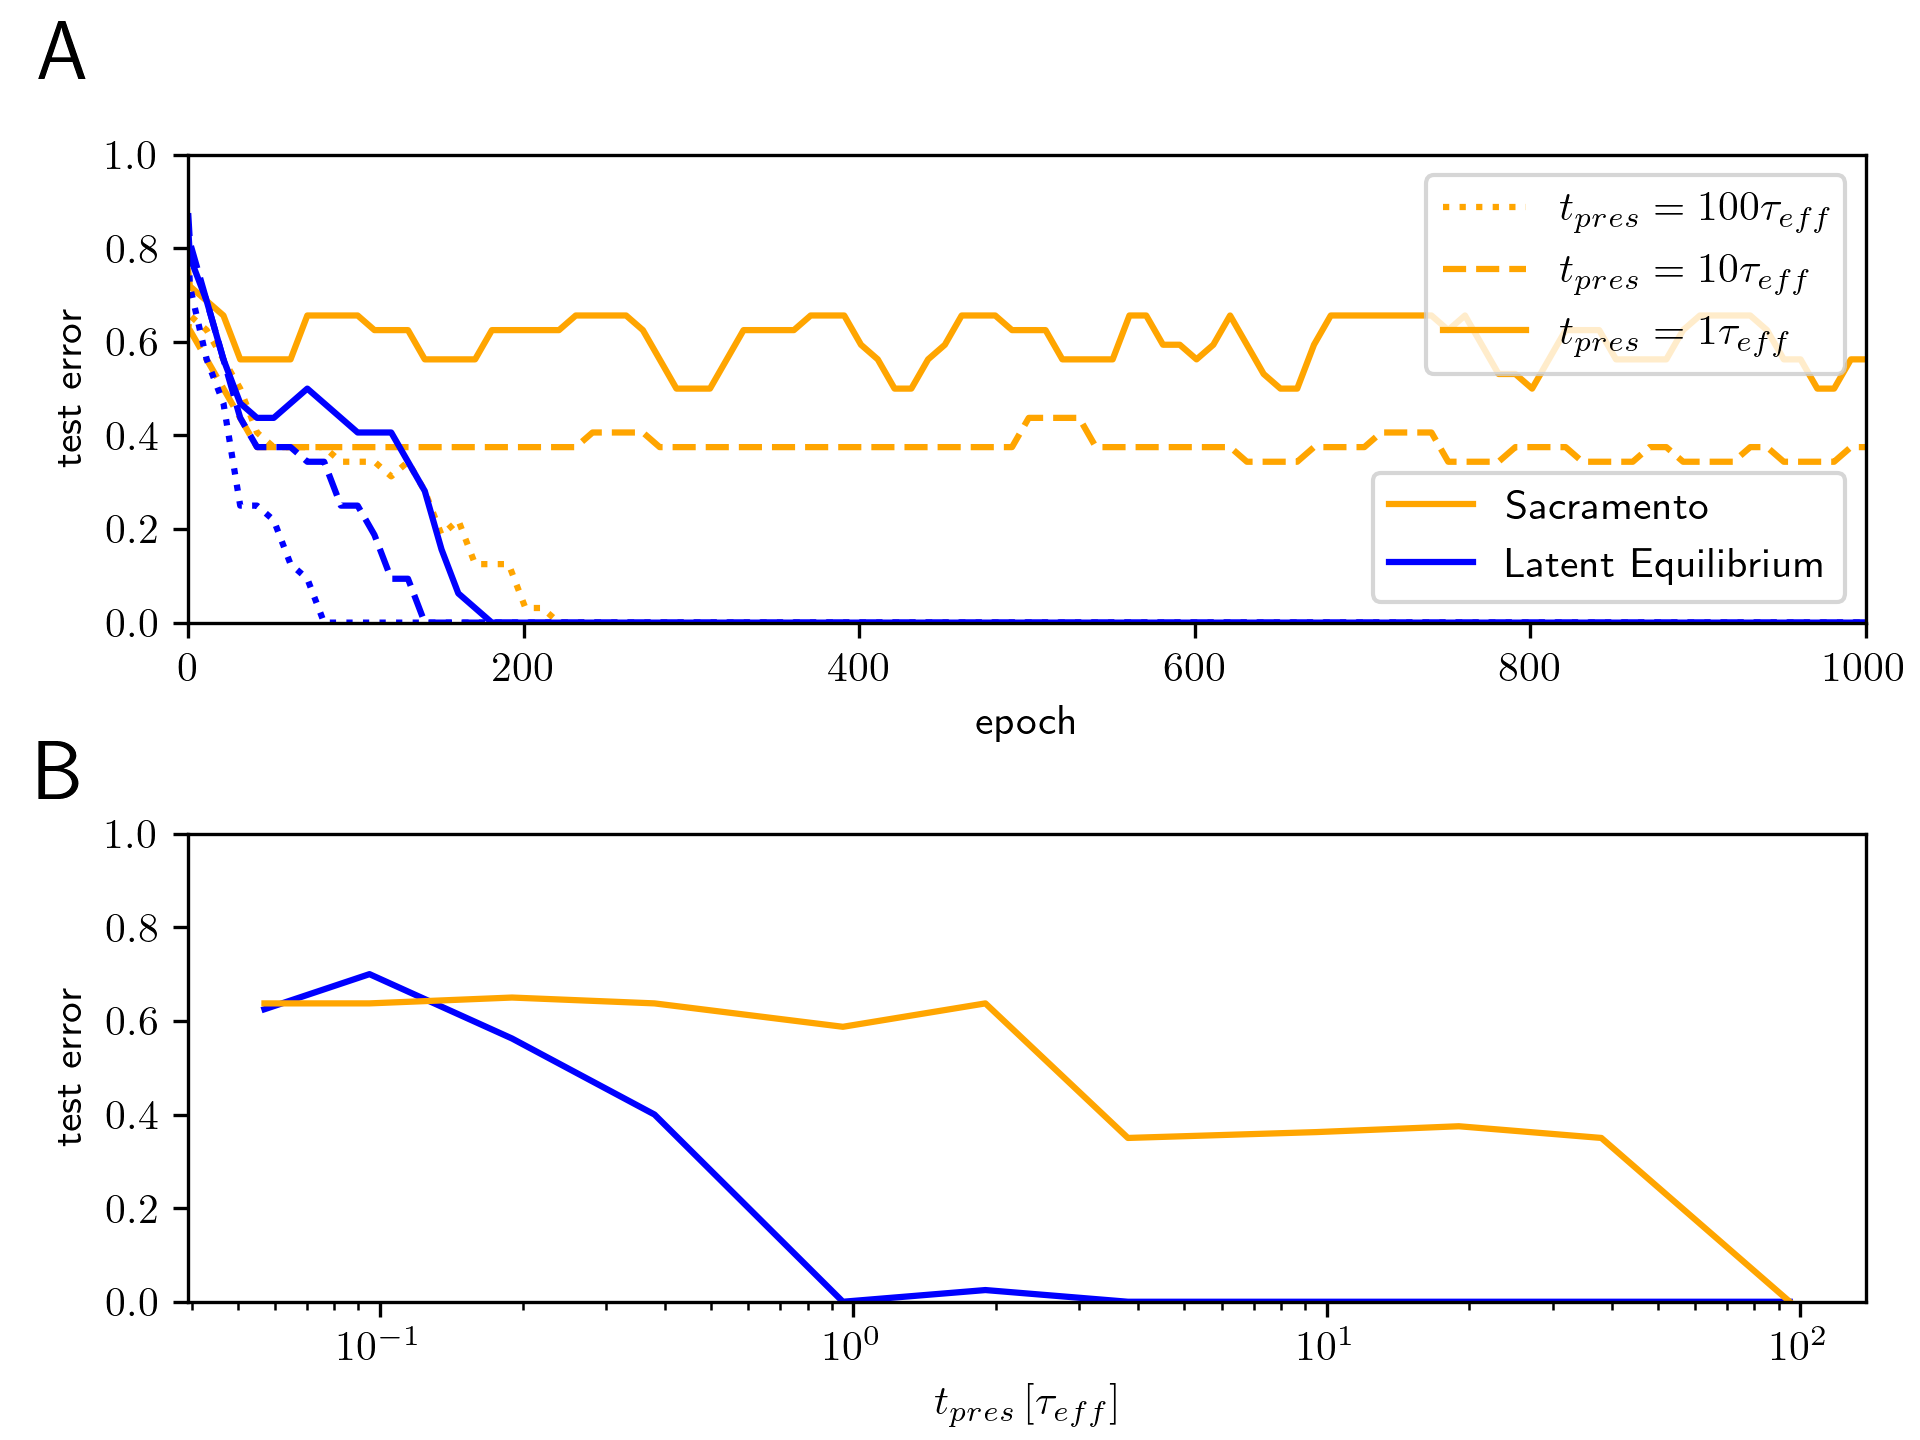
\includegraphics[width=0.9\textwidth]{fig_3_rnest}
  \caption[Replication of Fig. \ref{fig-bars-le-snest} using networks of rate neurons in the NEST simulator]{Replication
    of Fig. \ref{fig-bars-le-snest} using networks of rate neurons in the NEST simulator. A notable difference to the
    python implementation in Fig. \ref{fig-bars-le-numpy} is, that this version does not handle very low presentation
    times as well. This can likely be traced back to the synaptic delay enforced by NEST, which imposes an upper bound
    on network relaxation time. Besides that, performance of the two variants is very similar.}
  \label{fig-bars-le-rnest}
\end{figure}



\clearpage

\section{Supplementary Tables}



\renewcommand{\thetable}{S\arabic{table}}


\arrayrulecolor{white} % <--- {\renewcommand{\arraystretch}{1.45} 
\begin{table}[h]
  \resizebox{\textwidth}{!}{
    \begin{tabular}{|ll|ll|ll|} \hline \rowcolor[HTML]{B3B3B3} \multicolumn{2}{|l|}{\cellcolor[HTML]{B3B3B3}}      &
               \multicolumn{2}{l|}{\cellcolor[HTML]{B3B3B3}Temporal-error
               model}                                                                                          &
               \multicolumn{2}{l|}{\cellcolor[HTML]{B3B3B3}Explicit-error
               model}                                                                                                           \\
               \cline{3-6}
               \rowcolor[HTML]{B3B3B3}
               \multicolumn{2}{|l|}{\multirow{-2}{*}{\cellcolor[HTML]{B3B3B3}}}
                                                                                                               &
               \multicolumn{1}{l|}{\cellcolor[HTML]{B3B3B3}Contrastive
               learning}                                                                                       &
               Continuous
               update
                                                                                                               &
               \multicolumn{1}{l|}{\cellcolor[HTML]{B3B3B3}Predictive
               coding}                                                                                         &
               Dendritic error
               \\ \hline
               \rowcolor[HTML]{D9D9D9} \multicolumn{2}{|l|}{\cellcolor[HTML]{D9D9D9}Control signal}            &
               \multicolumn{1}{l|}{\cellcolor[HTML]{D9D9D9}{\color[HTML]{FE0000}
               Required}}                                                                                      &
               {\color[HTML]{FE0000}
                   Required}
                                                                                                               &
               \multicolumn{1}{l|}{\cellcolor[HTML]{D9D9D9}{\color[HTML]{32CB00}
               Not required}}                                                                                  &
               {\color[HTML]{32CB00}
                   Not required}
               \\ \hline
               \rowcolor[HTML]{D9D9D9}
               \multicolumn{2}{|l|}{\cellcolor[HTML]{D9D9D9}Connectivity}
                                                                                                               &
               \multicolumn{1}{l|}{\cellcolor[HTML]{D9D9D9}{\color[HTML]{32CB00}
                   Unconstrained}}
                                                                                                               &
               {\color[HTML]{32CB00}
               Unconstrained}                                                                                  &
               \multicolumn{1}{l|}{\cellcolor[HTML]{D9D9D9}{\color[HTML]{FE0000}
                   Constrained}}
                                                                                                               &
               {\color[HTML]{FE0000}
               Constrained}                                                                                                     \\
               \hline
               \rowcolor[HTML]{D9D9D9}
               \multicolumn{2}{|l|}{\cellcolor[HTML]{D9D9D9}Propagation
               time}                                                                                           &
               \multicolumn{1}{l|}{\cellcolor[HTML]{D9D9D9}{\color[HTML]{32CB00}
               L-1}}                                                                                           &
               {\color[HTML]{32CB00}
                   L-1}
                                                                                                               &
               \multicolumn{1}{l|}{\cellcolor[HTML]{D9D9D9}{\color[HTML]{FE0000}
               2L-1}}                                                                                          &
               {\color[HTML]{32CB00}
                   L-1}
               \\
               \hline \rowcolor[HTML]{D9D9D9} \multicolumn{2}{|l|}{\cellcolor[HTML]{D9D9D9}Pre-training}       &
               \multicolumn{1}{l|}{\cellcolor[HTML]{D9D9D9}{\color[HTML]{32CB00}
               Not required}}                                                                                  &
               {\color[HTML]{32CB00}
               Not required}                                                                                   &
               \multicolumn{1}{l|}{\cellcolor[HTML]{D9D9D9}{\color[HTML]{32CB00}
                   Not required}}
                                                                                                               &
               {\color[HTML]{FE0000}
               Required}                                                                                                        \\
               \hline
               \rowcolor[HTML]{D9D9D9}
               \multicolumn{2}{|l|}{\cellcolor[HTML]{D9D9D9}Error
               encoded in}                                                                                     &
               \multicolumn{1}{l|}{\cellcolor[HTML]{D9D9D9}\begin{tabular}[c]{@{}l@{}}Difference
                                                                   in activity \\
                                                                   between
                                                                   separate
                                                                   \\
                                                                   phases\end{tabular}}
                                                                                                               &
               \begin{tabular}[c]{@{}l@{}}Rate
                     of
                     change
                     of
                     \\
                     activity\end{tabular}
                                                                                                               &
               \multicolumn{1}{l|}{\cellcolor[HTML]{D9D9D9}\begin{tabular}[c]{@{}l@{}}Activity
                                                                   of
                                                                   specialised
                                                                   \\
                                                                   neurons\end{tabular}}                 &
               \begin{tabular}[c]{@{}l@{}}Apical dendrites of \\ pyramidal neurons\end{tabular}                  \\
               \hline \rowcolor[HTML]{D9D9D9} \multicolumn{2}{|l|}{\cellcolor[HTML]{D9D9D9}Data accounted for} &
               \multicolumn{1}{l|}{\cellcolor[HTML]{D9D9D9}\begin{tabular}[c]{@{}l@{}}Neural
                                                                   responses \\ and
                                                                   behaviour in a
                                                                   \\
                                                                   variety
                                                                   of
                                                                   tasks\end{tabular}}
                                                                                                               &
               \begin{tabular}[c]{@{}l@{}}Typical spike-time- \\ dependent plasticity\end{tabular}             &
               \multicolumn{1}{l|}{\cellcolor[HTML]{D9D9D9}\begin{tabular}[c]{@{}l@{}}Increased
                                                                   neural \\
                                                                   activity to
                                                                   \\
                                                                   unpredicted
                                                                   stimuli\end{tabular}}
                                                                                                               &
               \begin{tabular}[c]{@{}l@{}}Properties of \\
                     pyramidal neurons\end{tabular}                                                          \\
               \hline \rowcolor[HTML]{D9D9D9} \multicolumn{2}{|l|}{\cellcolor[HTML]{D9D9D9}MNIST performance}  &
               \multicolumn{1}{l|}{\cellcolor[HTML]{D9D9D9}$\sim$2-3}
                                                                                                               & -
                                                                                                               &
               \multicolumn{1}{l|}{\cellcolor[HTML]{D9D9D9}$\sim$1.7}
                                                                                                               & $\sim$1.96     \\
               \hline
    \end{tabular}
  }\caption[Comparison between biologically plausible approximations of Backprop]{Comparison between biologically
    plausible approximations of Backprop, adapted from \citep{whittington2019theories}. From left to right: Contrastive
    hebbian learning \citep{OReilly1996}, Contrastive learing with continuous update \citep{Bengio2017}, Predictive
    coding network \citep{Whittington2017}, Dendritic error network \citep{sacramento2018dendritic}. All algorithms were
    selected because they reflect some properties of biological brains, some of which are highlighted in the row "Data
    accounted for". All of the algorithms need to make concessions for this. In the first four rows, desirable
    properties are highlighted in green, while undesirable traits are highlighted in red.}\label{tab-wb-models}

\end{table}


\begin{table}
  \fontsize{12pt}{12pt}\selectfont
  \begin{center}
    \begin{tabular}{p{0.25\textwidth}p{0.6\textwidth}p{0.15\textwidth}}    \hline
      \textbf{Name}                & \textbf{Description}                                                        &
      \textbf{Default}
      \\
      \hline

      \\\textbf{Simulation} \\\hline
      \texttt{n\_epochs}           & Number of training iterations                                               &
      $1000$                                                                                                             \\
      \texttt{delta\_t}            & Euler integration step in [ms]                                              & $0.1$
      \\
      \texttt{t\_pres}             & Stimulus presentation time during training [ms]                             & $50$
      \\
      \texttt{out\_lag}            & Delay before recording output during testing [ms]                           & $35$
      \\
      \texttt{dims}                & Network dimensions, i.e. pyramidal neurons per layer                        & [9,
      30, 3]                                                                                                             \\
      \texttt{threads}             & Number of threads for parallel processing                                   & $8$
      \\
      \texttt{test\_interval}      & Test the network every N epochs                                             & $10$
      \\
      \texttt{record\_interval}    & Interval for storing membrane potentials [ms]                               & $1$
      \\
      \texttt{init\_self\_pred}    & Flag to initialize weights to self-predicting state                         &
      \texttt{True}
      \\
      \texttt{noise}               & Flag to apply noise to all somatic membrane potentials                      &
      \texttt{False}                                                                                                     \\
      \texttt{sigma}               & Standard deviation for membrane potential noise                             & 0.3
      \\
      \texttt{mode}                & Which dataset to train on. Choice between (bars, mnist, self-pred, teacher) & bars
      \\
      \texttt{store\_errors}       & Flag to compute and store apical and interneuron errors during training     &
      \texttt{False}
      \\
      \texttt{network\_type}       & Choice between (numpy, snest, rnest)                                        & snest
      \\
      \texttt{tau\_x}              & Network input filtering time constant [ms]                                  & 0.1
      \\
      \texttt{reset}               & Reset method between simulations (0=no reset, 1=soft reset, 2=hard reset)   & 2
      \\

      \\
      \textbf{Neurons}
      \\\hline
      \texttt{latent\_equilibrium} & Flag for whether to use prospective transfer functions                      &
      \texttt{True}
      \\
      \texttt{g\_l}                & Somatic leakage conductance [nS]                                            & 0.03
      \\
      \texttt{g\_a}                & Apical compartment coupling conductance [nS]                                & 0.06
      \\
      \texttt{g\_d}                & Basal compartment coupling conductance [nS]                                 & 0.1
      \\
      \texttt{g\_som}              & Output neuron nudging conductance [nS]                                      & 0.06
      \\
      \texttt{g\_l\_eff}           & Effective leakage conductance [nS]                                          &
      \texttt{g\_l+g\_d+g\_a}
      \\
      \\
      \texttt{g\_lk\_dnd}          & Dendritic leakage [nS]                                                      &
      \texttt{delta\_t}
      \\
      \texttt{t\_ref}              & Refractory period [ms]                                                      & 0.0
      \\
      \texttt{C\_m\_som}           & Somatic compartment membrane capacitance [pF]                               & 1.0
      \\
      \texttt{C\_m\_bas}           & Basal compartment membrane capacitance [pF]                                 & 1.0
      \\
      \texttt{C\_m\_api}           & Apical compartment membrane capacitance [pF]                                & 1.0
      \\
      \texttt{gamma}               & Linearly scales  activation function $\phi$                                 & 1.0
      \\
      \texttt{beta}                & Exponentially scales  activation function $\phi$                            & 1.0
      \\
      \texttt{theta}               & Shifts  activation function $\phi$                                          & 0.0
      \\

      \\
      \textbf{Synapses}
      \\\hline
      \texttt{wmin\_init}          & Min. initial synaptic weight                                                & -1.0
      \\
      \texttt{wmax\_init}          & Max. initial synaptic weight                                                & 1.0
      \\
      \texttt{Wmin}                & Min. allowed synaptic weight                                                & -4.0
      \\
      \texttt{Wmax}                & Max. allowed synaptic weight                                                & 4.0
      \\
      \texttt{tau\_delta}          & Weight change filter time constant (NEST only) [ms]                         & 1.0
      \\

      \texttt{p\_conn}             & Connection probability between populations                                  & 1.0
      \\
      \texttt{eta\_ip}             & Learning rate for $pyr\rightarrow intn$ synapses                            & 0.004
      \\
      \texttt{eta\_pi}             & Learning rate for $intn\rightarrow pyr$ synapses                            & 0.01
      \\
      \texttt{eta\_up}             & Learning rates for feedforwarsd $pyr\rightarrow pyr$ synapses               &
      [0.01, 0.003]                                                                                                      \\
      \texttt{eta\_down}           & Learning rate for feedback $pyr\rightarrow pyr$ synapses                    & 0.0
      \\
    \end{tabular}\caption{Default parameters for the dendritic error model. }\label{tab-params}
  \end{center}
\end{table}




\begin{enumerate}
  \item In the torch implementation, there no persistence between timesteps at all. Input is fed into the network and processed feedforward and feedback. Output is read and weights (+biases) are updated. Rinse and repeat.
  \item to what extent should dendritic and somatic compartments decay?
  \item Can (should) we transfer the learned bias from the torch model?
  \item I can "cheat" the apical voltage constraint for self prediction by increasing apical leakage conductance. How does this influence my model?
  \item Is there some analytical approach to identifying why synaptic weights deviate from their intended targets?
  \item I think that lambda needs to be scaled in dependence on $g_{lk}$, such that current inputs, spike inputs and leakage cancel each other out.

  \item How do we deal with population size dependence?

\end{enumerate}

\section{Parameter study}
\begin{itemize}

  \item Transfer function $\phi$
  \item interneuron mixing factor $\lambda$
  \item injected current $I_e$
  \item dendritic leakage conductance $g_{lk,d}$
  \item somatic leakage conductance $g_{lk,s}$
  \item Learning rate $\eta$
  \item synaptic time constants $\tau_{delta}$
  \item noise level $\sigma$
  \item Simulation time $\mathbb{T}$
  \item plasticity onset after the network relaxes
  \item compartment current decay $\tau_{syn}$

\end{itemize}


\subsection*{Observations}

\begin{itemize}
  \item In self-predicting paradigm, Apical errors stay constant, despite interneuron error steadily increasing.
  \item Interneuron error (between neuron pairs) is proportional to absolute somatic voltage in self-predicting paradigm.
  \item abs interneuron voltage is always higher than abs pyramidal voltage. This kind of makes sense, as interneurons receive direct current input proportional to pyramidal voltage in addition to feedforward input. This discrepancy disappears when setting $\lambda$ to 0 as expected.
  \item When plasticity is enabled from a random starting configuration, apical error \textbf{sometimes} converges to better values than can be achieved in both self-predicting paradigms. I believe this to be a huge issue: the self-predicting state does not cause minimal apical voltage, and completely decayed feedback weights are preferable to perfectly counteracting feedback weights.
  \item feedforward weights tend to increase absolutely, i.e. drift towards the closest extreme. \textit{This only happens since I re-implemented the second exponential term in the pyr\_synapse}. Yet they do not simply explode to the nearest extremum, but will traverse a zero weight to reach the maximum with equal sign as the weight they are supposed to match.
  \item feedback weights tend to decay to around zero. Yet they appear to remain close to zero in the direction they are supposed to be.
  \item Idea: I think that the somatic nudging is handled as straight currents being sent to the neuron, instead of the difference between actual and desired somatic voltage.
  \item In the paper and Mathematica code, Feedback learning rate is 2-5 times higher than feedforward lr. In my model, for learning to happen on similar time scales, feedback lr has to be ~100 times lower than feedforward lr. An indicator that my plasticity is messed up.
  \item The simulation is likely producing way too few spikes (5-20 per 1000ms iteration). Could adapting the activation function yield better results?
  \item In the Mathematica solution, leakage conductance is greater than 1! ($\delta U_i = -(g_L + g_D + g_{SI}) U_i + g_D V_{BI} + g_{SI} U_Y$) with $g_L + g_D + g_{SI} = 1.9$
\end{itemize}

\newpage

\chapter{Preliminary structural components}

\section{Synaptic delays}

Where I will inspect the implications of synaptic delays inherent to the NEST simulations on
the model and plasticity rule. In particular, I will look at the biological necessity for this
type of delay and discuss why any model attempting to replicate neuronal processes must be resilient
to these delays.


\section{Literature review - Backpropagation in SNN}

Where I will review other attempts at implementing biologically plausible Backpropagation
alternatives and contrast them to the current model.

\section{NEST Urbanczik-senn implementation}


\section{My neuron model}

\begin{itemize}
  \item Low pass filtering
  \item multi-compartment computation
  \item Imprecision of the ODE
  \item abuse of the somatic conductance
\end{itemize}

\subsection{NEST rate neuron shenanigans}

Given how long I worked on a rate neuron implementation in NEST, some pages should be devoted
to this effort.


\section{My synapse model}

Where I discuss the synapse implementation with regard to multi-compartment neurons,
urbanczik-archiving and in particular the issues with timing that arise from NEST delays.


\section{The relation between the pyramidal microcircuit and actual microcircuits}

Where I can finally use the shit that has been on my whiteboard for half a year...

This will also serve as valuable insight into how plausible this microcircuit actually is,
and might give some insight into possible model extensions.

\subsection{Interneurons and their jobs}

\section{Does it have to be backprop?}

Where I will explain my concerns regarding the usefulness of approximating backpropagation
in light of the substantial one-shot learning capability of the brain and the active inference
model.


\section{Discrepancies between mathematica and NEST model}

1. Weights deviate slightly. This difference can be alleviated by exposing a single stimulus for a longer duration before switching.

\section{Transfer functions}

Where I will discuss the sensitivity of this entire simulation to minor changes in the
parametrization and style of transfer function being used.

\chapter{The weight-leakage tradeoff}

Where I will discuss the issue, that decreasing both synaptic weights and dendritic leakage conductance
lead to more stability in the dendritic voltage, while at the same time requiring longer exposure
per iteration.


\section*{TODOs}

\begin{itemize}
  \item Prove that the network is stable in the self-predicting state and at the end of learning
  \item Show the limits of learning capability (i.e. how big of a network it can match)
  \item Test the network on a real-world dataset (mnist)
  \item prove/find literature on why the poisson process is a rate neuron in the limit.
  \item Does the network still learn when neurons have a refractory period?
  \item Comparison to other spiking backprops
  \item what can we learn from this? does it describe part of the brain
\end{itemize}

\newpage


\chapter{Open Questions}

\begin{itemize}
  \item Any tips for transitioning to large simulation? also regarding the threadripper
  \item Is refractoryness interesting to us or more of a sidenote?
  \item Neuron dropout?
  \item How does one prove that the network is converged and will not diverge again.
  \item randomized/longer synaptic delays?
  \item As a follow up of dropout, maybe even neurogenesis?
  \item Should I look at delaying injection of the target activation?
  \item more ways in which this is biologically implausible?
\end{itemize}

$t_{pres} 10 - 50 \tau$
\bibliography{bib/library.bib}

\end{document}